\documentclass[11pt,letterpaper,twocolumn]{fenbil}
\usepackage{amsmath}
\usepackage{amssymb}
\usepackage{graphicx}
\usepackage{tikz}
\title{FMM - Fizikte Matematiksel Metotlar - Ders Notları}
\author{Celal Ekrem Torun}
\date{6 Mart 2025}

\begin{document}
\twocolumn[\begin{@twocolumnfalse}

\begin{minipage}{0.15\textwidth}{
    }
\end{minipage}
\hspace{25pt}
\begin{minipage}{0.75\textwidth}
\vspace{5mm}
\Large{\textbf{FMM - Fizikte Matematiksel Metotlar - Ders 1 (6 Mart 2025)}}
    \vspace{3mm}
    
    \large{\textbf{Hazırlayan}; Celal Ekrem Torun}
    \vspace{2mm}
    
    \fontsize{0.35cm}{0.5cm}\selectfont \textit{Fizik Bölümü, İstanbul Üniversitesi\newline 
    Beyazıt, Fatih, İstanbul, Türkiye}
    
\end{minipage}

\small

\end{@twocolumnfalse}]

\section{Matematiksel Metotlar}

\textbf{Not:} 1 Mart'ta gradyen vektörü işlendi, 6 Mart'ta eğrisel koordinatlara başlanacak.

\subsection{Gradyen}

\textbf{Tanım:} Bir $\phi(x, y, z)$ skaler alanının gradyeni, o alanın en hızlı değişim yönünü ve büyüklüğünü gösteren bir vektör alanıdır.

Kartezyen koordinatlarda gradyen şu şekilde tanımlanır:

\[
\nabla \phi = \frac{\partial \phi}{\partial x} \hat{e_x} + \frac{\partial \phi}{\partial y} \hat{e_y} + \frac{\partial \phi}{\partial z} \hat{e_z}
\]

Burada:

\begin{itemize}
    \item $\nabla \phi$: Gradyen vektörü
    \item $\phi(x, y, z)$: Skaler alan
    \item $\hat{e_x}$, $\hat{e_y}$, $\hat{e_z}$: Sırasıyla $x$, $y$ ve $z$ yönlerindeki birim vektörler
\end{itemize}

\textbf{Önemli Not:} $\nabla \phi$, $\hat{e_x}$, $\hat{e_y}$ ve $\hat{e_z}$ ile ayrı ayrı skalar çarpılırsa, $\phi$ fonksiyonunun sınırları ile $x$, $y$ ve $z$ doğrultusundaki değişimi bulunur.

Bir $P(x,y,z)$ noktasındaki $\phi$ fonksiyonunun değişim oranı, $\nabla \phi \cdot d\vec{r}$ ile bulunur. Burada $d\vec{r}$, $P$ noktasından küçük bir yer değiştirmeyi temsil eden vektördür. Eğer $\phi = c_1$ yüzeyinden $\phi = c_2$ yüzeyine gidilirse, değişim $d\phi = c_2 - c_1$ olur ve $d\phi \neq 0$ olur.

Eğer $\nabla \phi \cdot d\vec{r} = d\phi = 0$ ise, $\nabla \phi$, $d\vec{r}$ vektörüne diktir. Bu durumda $\nabla \phi$, $\frac{\nabla \phi}{|\nabla \phi|}$ ile aynı yöndedir.

\subsection{Doğrultu Türevi}

\textbf{Tanım:} Bir $\phi(x,y,z)$ skaler alanının, bir $\vec{u}$ birim vektörü yönündeki doğrultu türevi, $\phi$'nin $\vec{u}$ yönündeki değişim oranını verir.

Doğrultu türevi şu şekilde tanımlanır:

\[
\frac{\partial \phi}{\partial u} = \nabla \phi \cdot \hat{u} = |\nabla \phi| |\hat{u}| \cos \theta
\]

Burada:
\begin{itemize}
    \item $\frac{\partial \phi}{\partial u}$: Doğrultu türevi
    \item $\nabla \phi$: Gradyen vektörü
    \item $\hat{u}$: Birim vektör
    \item $\theta$: $\nabla \phi$ ve $\hat{u}$ arasındaki açı
\end{itemize}

$\frac{\partial \phi}{\partial u}$, $\phi$'nin bir $P(x,y,z)$ noktasındaki $\vec{u}$ birim vektörü ile belirlenen doğrultudaki doğrultu türevidir.

$\frac{\partial \phi}{\partial u} = \nabla \phi \cdot \hat{u} = |\nabla \phi| \cos \theta$

\subsection{Örnek Soru}

$\phi(x, y, z) = x^2yz + 4z^2$ fonksiyonunun $P(1, -2, -1)$ noktasındaki $\vec{dr} = (2\hat{e_x} - \hat{e_y} - 2\hat{e_z})$ doğrultusundaki türevini bulun.

\textbf{Çözüm:}

\textit{Adım 1: Gradyeni hesaplayalım:}

$\nabla \phi = (2xyz) \hat{e_x} + (x^2z) \hat{e_y} + (x^2y + 8z) \hat{e_z}$

\textit{Adım 2: P(1, -2, -1) noktasındaki gradyeni hesaplayalım:}

$\nabla \phi |_P = (2(1)(-2)(-1)) \hat{e_x} + ((1)^2(-1)) \hat{e_y} + ((1)^2(-2) + 8(-1)) \hat{e_z} = 4 \hat{e_x} - \hat{e_y} - 10 \hat{e_z}$

\textit{Adım 3: $\vec{u}$ birim vektörünü bulalım:}

$|\vec{dr}| = \sqrt{2^2 + (-1)^2 + (-2)^2} = \sqrt{9} = 3$

$\hat{u} = \frac{\vec{dr}}{|\vec{dr}|} = \frac{2}{3} \hat{e_x} - \frac{1}{3} \hat{e_y} - \frac{2}{3} \hat{e_z}$

\textit{Adım 4: Doğrultu türevini hesaplayalım:}

$\frac{\partial \phi}{\partial u} = \nabla \phi \cdot \hat{u} = (4 \hat{e_x} - \hat{e_y} - 10 \hat{e_z}) \cdot (\frac{2}{3} \hat{e_x} - \frac{1}{3} \hat{e_y} - \frac{2}{3} \hat{e_z}) = \frac{8}{3} + \frac{1}{3} + \frac{20}{3} = \frac{29}{3} \approx 9.67$

\subsection{Eğrisel Koordinatlar}

Üç boyutlu Öklit uzayında, bir noktanın Kartezyen koordinatları $(x, y, z)$ ile ifade edilir. Şimdi, bu koordinatlara bağlı üç yeni değişken tanımlayalım:

\begin{equation}
u_1 = u_1(x, y, z)
\end{equation}
\begin{equation}
u_2 = u_2(x, y, z)
\end{equation}
\begin{equation}
u_3 = u_3(x, y, z)
\end{equation}

Bu yeni değişkenler, eğrisel koordinatları temsil eder.

\subsubsection{$u_1$, $u_2$, $u_3$'ün Bağımsız Fonksiyonlar Olması}

Lineer homojen bir sistemin sıfırdan farklı çözüme sahip olabilmesi için, katsayılar determinantının sıfıra eşit olması gerekmektedir. Şimdi, $u_1$, $u_2$, $u_3$'ün bağımsız fonksiyonlar olmasının ne anlama geldiğini inceleyelim.

$u_1(x, y, z)$, $u_2(x, y, z)$ ve $u_3(x, y, z)$ fonksiyonları için aşağıdaki ifadeler tanımlanır:

\begin{equation}
u_1 = u_1(x, y, z)
\end{equation}
\begin{equation}
u_2 = u_2(x, y, z)
\end{equation}
\begin{equation}
u_3 = u_3(x, y, z)
\end{equation}

Bu fonksiyonların diferansiyelleri ise şu şekildedir:

\begin{equation}
du_1 = \frac{\partial u_1}{\partial x} dx + \frac{\partial u_1}{\partial y} dy + \frac{\partial u_1}{\partial z} dz
\end{equation}
\begin{equation}
du_2 = \frac{\partial u_2}{\partial x} dx + \frac{\partial u_2}{\partial y} dy + \frac{\partial u_2}{\partial z} dz
\end{equation}
\begin{equation}
du_3 = \frac{\partial u_3}{\partial x} dx + \frac{\partial u_3}{\partial y} dy + \frac{\partial u_3}{\partial z} dz
\end{equation}

Bu denklemleri matris formunda ifade edebiliriz:

\begin{equation}
\begin{bmatrix} du_1 \\ du_2 \\ du_3 \end{bmatrix} = 
\begin{bmatrix}
\frac{\partial u_1}{\partial x} & \frac{\partial u_1}{\partial y} & \frac{\partial u_1}{\partial z} \\
\frac{\partial u_2}{\partial x} & \frac{\partial u_2}{\partial y} & \frac{\partial u_2}{\partial z} \\
\frac{\partial u_3}{\partial x} & \frac{\partial u_3}{\partial y} & \frac{\partial u_3}{\partial z}
\end{bmatrix}
\begin{bmatrix} dx \\ dy \\ dz \end{bmatrix}
\end{equation}

Bu matrisi daha kompakt bir şekilde ifade etmek için, aşağıdaki tanımlamaları yapalım:

\begin{equation}
d\mathbf{u} = \begin{bmatrix} du_1 \\ du_2 \\ du_3 \end{bmatrix}, \quad
A = \begin{bmatrix}
\frac{\partial u_1}{\partial x} & \frac{\partial u_1}{\partial y} & \frac{\partial u_1}{\partial z} \\
\frac{\partial u_2}{\partial x} & \frac{\partial u_2}{\partial y} & \frac{\partial u_2}{\partial z} \\
\frac{\partial u_3}{\partial x} & \frac{\partial u_3}{\partial y} & \frac{\partial u_3}{\partial z}
\end{bmatrix}, \quad
d\mathbf{x} = \begin{bmatrix} dx \\ dy \\ dz \end{bmatrix}
\end{equation}

Bu durumda, yukarıdaki denklem şu şekilde yazılabilir:

\begin{equation}
d\mathbf{u} = A \, d\mathbf{x}
\end{equation}

$dx$, $dy$ ve $dz$'yi $du_1$, $du_2$ ve $du_3$ cinsinden ifade etmek için, $A$ matrisinin tersini almamız gerekir:

\begin{equation}
d\mathbf{x} = A^{-1} \, d\mathbf{u}
\end{equation}

$A^{-1}$ matrisinin var olabilmesi için, $A$ matrisinin determinantı sıfırdan farklı olmalıdır:

\begin{equation}
J = \det(A) \neq 0
\end{equation}

Burada $J$, Jacobian determinantıdır. $A^{-1}$ matrisi, $A$'nın ek matrisinin determinantına bölünmesiyle bulunur:

\begin{equation}
A^{-1} = \frac{\text{adj}(A)}{J}
\end{equation}

Bu durumda, $dx$, $dy$ ve $dz$ aşağıdaki şekilde ifade edilebilir:

\begin{equation}
\begin{bmatrix} dx \\ dy \\ dz \end{bmatrix} = A^{-1} \begin{bmatrix} du_1 \\ du_2 \\ du_3 \end{bmatrix}
\end{equation}

Kartezyen koordinatları eğrisel koordinatlar cinsinden ifade etmek için, aşağıdaki bağıntıları kullanırız:

\begin{equation}
x = x(u_1, u_2, u_3)
\end{equation}
\begin{equation}
y = y(u_1, u_2, u_3)
\end{equation}
\begin{equation}
z = z(u_1, u_2, u_3)
\end{equation}

Bu durumda, konum vektörü $\vec{r}$ aşağıdaki gibi ifade edilir:

\begin{equation}
\vec{r} = x(u_1, u_2, u_3) \, \hat{e_x} + y(u_1, u_2, u_3) \, \hat{e_y} + z(u_1, u_2, u_3) \, \hat{e_z}
\end{equation}

\subsubsection{Eğrisel Koordinatların Geometrik Gösterimi}

Aşağıdaki şemalar, eğrisel koordinatların ve Kartezyen koordinat sisteminin ayrı ayrı gösterimlerini sunmaktadır.

\textbf{Kartezyen Koordinat Sistemi:}

\begin{figure}[htbp]
    \centering
    \begin{tikzpicture}
        \draw[thick, ->] (-3,0) -- (3,0) node[anchor=north west] {x};
        \draw[thick, ->] (0,-3) -- (0,3) node[anchor=south east] {y};
        \draw[thick, ->] (0,0) -- (1.5,1.5) node[anchor=west] {z};
        
        \node[below right] at (2.2, -0.2) {Apsis (x)};
        \node[above] at (-2.2, 0) {Ordinat (y)};
    \end{tikzpicture}
    \caption{Kartezyen Koordinat Sistemi}
    \label{fig:kartezyen_koordinat}
\end{figure}

Bu şemada:

\begin{itemize}
    \item \textit{Apsis (x)}: Yatay ekseni temsil eder.
    \item \textit{Ordinat (y)}: Dikey ekseni temsil eder.
    \item \textit{Kot (z)}: Derinlik eksenini temsil eder.
\end{itemize}

\textbf{Eğrisel Koordinat Sistemi Gösterimi:}

\begin{figure}[htbp]
    \centering
    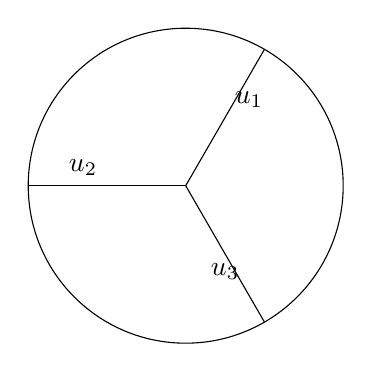
\begin{tikzpicture}
        \draw (0,0) circle (2cm);
        \draw (0,0) -- (60:2cm) node[midway, above right] {$u_1$};
        \draw (0,0) -- (180:2cm) node[midway, above left] {$u_2$};
        \draw (0,0) -- (300:2cm) node[midway, below] {$u_3$};
    \end{tikzpicture}
    \caption{Eğrisel Koordinat Sistemi}
    \label{fig:egrisel_koordinat}
\end{figure}

Bu şema, eğrisel koordinatları $(u_1, u_2, u_3)$ temsil eden bir dairesel gösterim sunar. Bu gösterim, eğrisel koordinatların Kartezyen koordinat sistemi ile ilişkisini anlamak için kullanılabilir.

Eğrisel koordinatlar, belirli bir probleme daha uygun bir koordinat sistemi seçme esnekliği sağlar. Örneğin, silindirik veya küresel koordinatlar, belirli simetrilere sahip problemleri çözmek için daha uygun olabilir.

\subsection{Eğrisel Koordinat Örnekleri}

\subsubsection{Silindirik Koordinatlar $(\rho, \phi, z)$}

Silindirik koordinatlar, üç boyutlu uzayı tanımlamak için kullanılan bir koordinat sistemidir. Bu sistemde, bir noktanın konumu, bir eksene olan uzaklığı $(\rho)$, bu eksen etrafındaki açısı $(\phi)$ ve eksen üzerindeki yüksekliği $(z)$ ile belirlenir.

\textbf{Tanımlar:}

\begin{itemize}
    \item \textit{$\rho$ (rho)}: $xy$ düzlemindeki orijinden olan uzaklık.
    \item \textit{$\phi$ (phi)}: $x$ ekseni ile $\rho$ arasındaki açı (azimut açısı).
    \item \textit{$z$}: $z$ ekseni üzerindeki yükseklik.
\end{itemize}

\textbf{Kartezyen ve Silindirik Koordinatlar Arasındaki İlişki:}

Kartezyen koordinatlardaki $(x, y, z)$ noktası ile silindirik koordinatlardaki $(\rho, \phi, z)$ noktası arasındaki dönüşüm aşağıdaki gibidir:

\begin{itemize}
    \item $x = \rho \cos \phi$
    \item $y = \rho \sin \phi$
    \item $z = z$
\end{itemize}

\textbf{Dönüşümün Tersi:}

\begin{itemize}
    \item $\rho = \sqrt{x^2 + y^2}$
    \item $\phi = \arctan \left( \frac{y}{x} \right)$
    \item $z = z$
\end{itemize}

\textbf{Geometrik Gösterim:}

\begin{figure}[htbp]
    \centering
    \begin{tikzpicture}
        % Eksenleri çiz
        \draw[thick, ->] (-3,0) -- (3,0) node[anchor=north west] {x};
        \draw[thick, ->] (0,-3) -- (0,3) node[anchor=south east] {y};
        \draw[thick, ->] (0,0) -- (1.5,1.5) node[anchor=west] {z};

        % Silindir çiz
        \draw[dashed] (1,0) arc (0:360:1);
        \draw[dashed] (1,0) -- (1,2);
        \draw[dashed] (-1,0) -- (-1,2);
        \draw[dashed] (1,2) arc (0:360:1);

        % P noktası
        \node[circle, fill, inner sep=1.5pt, label=above right:$P$] (P) at (0.7, 1, 1) {};

        % P' noktası
        \node[circle, fill, inner sep=1.5pt, label=below:$P'$] (Pp) at (0.7,0,0) {};

        % rho
        \draw[dashed] (0,0) -- (Pp) node[midway, below] {$\rho$};

        % z
        \draw[dashed] (Pp) -- (P) node[midway, right] {$z$};

        % Açı phi
        \draw (0.4,0) arc (0:45:0.4);
        \node at (0.7,0.3) {$\phi$};

    \end{tikzpicture}
    \caption{Silindirik Koordinat Sistemi}
    \label{fig:silindirik_koordinat}
\end{figure}

Bu şemada:

\begin{itemize}
    \item $P$: Uzaydaki bir noktayı temsil eder.
    \item $P'$: $P$ noktasının $xy$ düzlemindeki izdüşümüdür.
    \item $\rho$: $P'$ noktasının orijine olan uzaklığıdır.
    \item $\phi$: $x$ ekseni ile $OP'$ arasındaki açıdır (azimut açısı).
    \item $z$: $P$ noktasının $z$ ekseni üzerindeki yüksekliğidir.
\end{itemize}

\textbf{Jacobian Dönüşümü:}

Silindirik koordinatlardaki $(\rho, \phi, z)$ ile Kartezyen koordinatlardaki $(x, y, z)$ arasındaki ilişki aşağıdaki gibidir:

\begin{itemize}
    \item $x = \rho \cos \phi$
    \item $y = \rho \sin \phi$
    \item $z = z$
\end{itemize}

Burada $\phi$, azimut açısını temsil etmektedir.

Bu dönüşümü ifade etmek için Jacobian matrisini kullanabiliriz. Jacobian matrisi, koordinat dönüşümünün kısmi türevlerini içerir:

\begin{equation}
J = \begin{bmatrix}
\frac{\partial x}{\partial \rho} & \frac{\partial x}{\partial \phi} & \frac{\partial x}{\partial z} \\
\frac{\partial y}{\partial \rho} & \frac{\partial y}{\partial \phi} & \frac{\partial y}{\partial z} \\
\frac{\partial z}{\partial \rho} & \frac{\partial z}{\partial \phi} & \frac{\partial z}{\partial z}
\end{bmatrix}
\end{equation}

Bu matrisin elemanlarını hesaplarsak:

\begin{itemize}
    \item $\frac{\partial x}{\partial \rho} = \cos \phi$
    \item $\frac{\partial x}{\partial \phi} = -\rho \sin \phi$
    \item $\frac{\partial x}{\partial z} = 0$
    \item $\frac{\partial y}{\partial \rho} = \sin \phi$
    \item $\frac{\partial y}{\partial \phi} = \rho \cos \phi$
    \item $\frac{\partial y}{\partial z} = 0$
    \item $\frac{\partial z}{\partial \rho} = 0$
    \item $\frac{\partial z}{\partial \phi} = 0$
    \item $\frac{\partial z}{\partial z} = 1$
\end{itemize}

Bu değerleri Jacobian matrisine yerleştirdiğimizde:

\begin{equation}
J = \begin{bmatrix}
\cos \phi & -\rho \sin \phi & 0 \\
\sin \phi & \rho \cos \phi & 0 \\
0 & 0 & 1
\end{bmatrix}
\end{equation}

Jacobian determinantı ise şu şekilde hesaplanır:

\begin{equation}
\det(J) = \rho \cos^2 \phi + \rho \sin^2 \phi = \rho (\cos^2 \phi + \sin^2 \phi) = \rho
\end{equation}

Burada $\rho = \sqrt{x^2 + y^2}$ ve $\rho \neq 0$ olmalıdır.

Ayrıca, $\phi = \arctan \left( \frac{y}{x} \right)$ ifadesi kullanılır.

$z = z$ olduğundan, $z$ için türev dönüşümleri basittir.

Bu Jacobian determinantı, hacim elemanının dönüşümünde kullanılır:

\begin{equation}
dV = dx \, dy \, dz = |J| \, d\rho \, d\phi \, dz = \rho \, d\rho \, d\phi \, dz
\end{equation}

Bu dönüşümler, koordinatları bir sistemden diğerine dönüştürmek için kullanılır. Jacobian determinantı, dönüşümün hacim elemanını nasıl etkilediğini gösterir.

\subsection{Eğrisel Koordinat Sisteminin Taban Vektörleri ve Ölçek Çarpanları}

Eğrisel koordinat sistemlerinde, taban vektörleri ve ölçek çarpanları, koordinat sisteminin geometrik özelliklerini anlamak için önemlidir. Bu bölümde, bu kavramları detaylı bir şekilde inceleyeceğiz.

\textbf{1. Taban Vektörlerinin Tanımı:}

Eğrisel koordinatlarda, taban vektörleri, her bir koordinatın değişim yönünü gösterir. Örneğin, $(u_1, u_2, u_3)$ eğrisel koordinat sisteminde, taban vektörleri şu şekilde tanımlanır:

\begin{itemize}
    \item $\vec{e_1} = \frac{\partial \vec{r}}{\partial u_1}$: $u_1$ koordinatının değişim yönündeki taban vektörü.
    \item $\vec{e_2} = \frac{\partial \vec{r}}{\partial u_2}$: $u_2$ koordinatının değişim yönündeki taban vektörü.
    \item $\vec{e_3} = \frac{\partial \vec{r}}{\partial u_3}$: $u_3$ koordinatının değişim yönündeki taban vektörü.
\end{itemize}

Burada $\vec{r}$, konum vektörünü temsil eder.

\textbf{2. Geometrik Gösterim:}

Aşağıdaki şema, $u_1$, $u_2$ ve $u_3$ koordinatlarını düzlemsel olarak göstermektedir. Bu gösterimde, her bir koordinat, eski Windows logosuna benzer şekilde, farklı düzlemleri temsil etmektedir.

\begin{figure}[htbp]
    \centering
    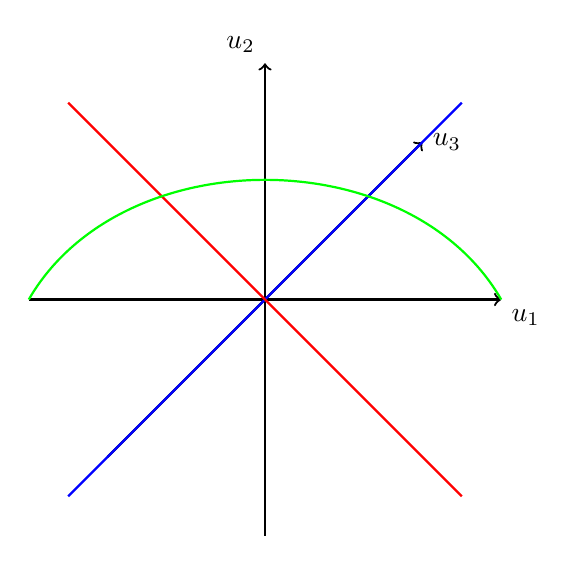
\begin{tikzpicture}
        % Eksenleri çiz
        \draw[thick, ->] (-3,0) -- (3,0) node[anchor=north west] {$u_1$};
        \draw[thick, ->] (0,-3) -- (0,3) node[anchor=south east] {$u_2$};
        \draw[thick, ->] (-2,-2) -- (2,2) node[anchor=west] {$u_3$};

        % Eğrisel yüzeyler
        \draw[blue, thick] (-2.5, -2.5) to[out=45,in=-135] (2.5,2.5);
        \draw[red, thick] (-2.5, 2.5) to[out=-45,in=135] (2.5,-2.5);
        \draw[green, thick] (-3,0) to[out=60,in=120] (3,0);
    \end{tikzpicture}
    \caption{Eğrisel Koordinat Sistemi Taban Vektörleri}
    \label{fig:egrisel_taban_vektorleri}
\end{figure}

Bu şemada, $u_1$, $u_2$ ve $u_3$ koordinatları, farklı düzlemleri temsil etmektedir. Bu düzlemlerin kesişimi, uzaydaki bir noktayı tanımlar.

\textbf{3. Taylor Serisi Açılımı:}

Şimdi, $u_2$ ve $u_3$ koordinatlarını sabit tutup, $u_1$ koordinatına $du_1$ artışı verelim. Bu durumda, yeni noktamız $P_1(u_1 + du_1, u_2, u_3)$ olacaktır. $P(u_1, u_2, u_3)$ noktasından $P_1$ noktasına olan vektör:

\begin{equation}
d\vec{r_1} = \vec{r}(u_1 + du_1, u_2, u_3) - \vec{r}(u_1, u_2, u_3)
\end{equation}

Bu ifadeyi Taylor serisine açarsak:

\begin{equation}
\vec{r}(u_1 + du_1, u_2, u_3) = \vec{r}(u_1, u_2, u_3) + \frac{\partial \vec{r}}{\partial u_1} du_1 + O(du_1^2)
\end{equation}

Burada $O(du_1^2)$, $du_1$'in ikinci ve daha yüksek dereceli terimlerini temsil eder. Bu terimleri ihmal edersek:

\begin{equation}
d\vec{r_1} = \frac{\partial \vec{r}}{\partial u_1} du_1 = \vec{e_1} du_1
\end{equation}

Benzer şekilde, diğer koordinatlar için de aynı işlemi yapabiliriz:

\begin{itemize}
    \item $d\vec{r_2} = \frac{\partial \vec{r}}{\partial u_2} du_2 = \vec{e_2} du_2$
    \item $d\vec{r_3} = \frac{\partial \vec{r}}{\partial u_3} du_3 = \vec{e_3} du_3$
\end{itemize}

Bu durumda, $d\vec{r}$ vektörü:

\begin{equation}
d\vec{r} = \frac{\partial \vec{r}}{\partial u_1} du_1 + \frac{\partial \vec{r}}{\partial u_2} du_2 + \frac{\partial \vec{r}}{\partial u_3} du_3 = \vec{e_1} du_1 + \vec{e_2} du_2 + \vec{e_3} du_3
\end{equation}

\textbf{4. Ölçek Çarpanları:}

Ölçek çarpanları, her bir koordinatın değişiminin, uzunluk birimindeki değişime nasıl dönüştüğünü gösterir. Ölçek çarpanları şu şekilde tanımlanır:

\begin{itemize}
    \item $h_1 = |\vec{e_1}| = \left| \frac{\partial \vec{r}}{\partial u_1} \right|$
    \item $h_2 = |\vec{e_2}| = \left| \frac{\partial \vec{r}}{\partial u_2} \right|$
    \item $h_3 = |\vec{e_3}| = \left| \frac{\partial \vec{r}}{\partial u_3} \right|$
\end{itemize}

Bu durumda, $d\vec{r}$ vektörünün uzunluğu:

\begin{equation}
ds^2 = (h_1 du_1)^2 + (h_2 du_2)^2 + (h_3 du_3)^2
\end{equation}

Bu ifade, eğrisel koordinatlardaki uzunluk elemanını temsil eder.

\textbf{5. Özet:}

Bu bölümde, eğrisel koordinat sistemlerinin taban vektörlerini, ölçek çarpanlarını ve uzunluk elemanını nasıl hesaplayacağımızı öğrendik. Bu kavramlar, eğrisel koordinat sistemlerindeki geometrik hesaplamalar için önemlidir.

\end{document}
\documentclass[11pt,letterpaper,twocolumn]{fenbil}
\usepackage{amsmath}
\usepackage{amssymb}
\usepackage{graphicx}
\usepackage{tikz}
\title{FMM - Fizikte Matematiksel Metotlar - Ders Notları}
\author{Celal Ekrem Torun}
\date{6 Mart 2025}

\begin{document}
\twocolumn[\begin{@twocolumnfalse}

\begin{minipage}{0.15\textwidth}{
    }
\end{minipage}
\hspace{25pt}
\begin{minipage}{0.75\textwidth}
\vspace{5mm}
\Large{\textbf{FMM - Fizikte Matematiksel Metotlar - Ders 1 (6 Mart 2025)}}
    \vspace{3mm}
    
    \large{\textbf{Hazırlayan}; Celal Ekrem Torun}
    \vspace{2mm}
    
    \fontsize{0.35cm}{0.5cm}\selectfont \textit{Fizik Bölümü, İstanbul Üniversitesi\newline 
    Beyazıt, Fatih, İstanbul, Türkiye}
    
\end{minipage}

\small

\end{@twocolumnfalse}]

\section{Matematiksel Metotlar}

\textbf{Not:} 1 Mart'ta gradyen vektörü işlendi, 6 Mart'ta eğrisel koordinatlara başlanacak.

\subsection{Gradyen}

\textbf{Tanım:} Bir $\phi(x, y, z)$ skaler alanının gradyeni, o alanın en hızlı değişim yönünü ve büyüklüğünü gösteren bir vektör alanıdır.

Kartezyen koordinatlarda gradyen şu şekilde tanımlanır:

\[
\nabla \phi = \frac{\partial \phi}{\partial x} \hat{e_x} + \frac{\partial \phi}{\partial y} \hat{e_y} + \frac{\partial \phi}{\partial z} \hat{e_z}
\]

Burada:

\begin{itemize}
    \item $\nabla \phi$: Gradyen vektörü
    \item $\phi(x, y, z)$: Skaler alan
    \item $\hat{e_x}$, $\hat{e_y}$, $\hat{e_z}$: Sırasıyla $x$, $y$ ve $z$ yönlerindeki birim vektörler
\end{itemize}

\textbf{Önemli Not:} $\nabla \phi$, $\hat{e_x}$, $\hat{e_y}$ ve $\hat{e_z}$ ile ayrı ayrı skalar çarpılırsa, $\phi$ fonksiyonunun sınırları ile $x$, $y$ ve $z$ doğrultusundaki değişimi bulunur.

Bir $P(x,y,z)$ noktasındaki $\phi$ fonksiyonunun değişim oranı, $\nabla \phi \cdot d\vec{r}$ ile bulunur. Burada $d\vec{r}$, $P$ noktasından küçük bir yer değiştirmeyi temsil eden vektördür. Eğer $\phi = c_1$ yüzeyinden $\phi = c_2$ yüzeyine gidilirse, değişim $d\phi = c_2 - c_1$ olur ve $d\phi \neq 0$ olur.

Eğer $\nabla \phi \cdot d\vec{r} = d\phi = 0$ ise, $\nabla \phi$, $d\vec{r}$ vektörüne diktir. Bu durumda $\nabla \phi$, $\frac{\nabla \phi}{|\nabla \phi|}$ ile aynı yöndedir.

\subsection{Doğrultu Türevi}

\textbf{Tanım:} Bir $\phi(x,y,z)$ skaler alanının, bir $\vec{u}$ birim vektörü yönündeki doğrultu türevi, $\phi$'nin $\vec{u}$ yönündeki değişim oranını verir.

Doğrultu türevi şu şekilde tanımlanır:

\[
\frac{\partial \phi}{\partial u} = \nabla \phi \cdot \hat{u} = |\nabla \phi| |\hat{u}| \cos \theta
\]

Burada:
\begin{itemize}
    \item $\frac{\partial \phi}{\partial u}$: Doğrultu türevi
    \item $\nabla \phi$: Gradyen vektörü
    \item $\hat{u}$: Birim vektör
    \item $\theta$: $\nabla \phi$ ve $\hat{u}$ arasındaki açı
\end{itemize}

$\frac{\partial \phi}{\partial u}$, $\phi$'nin bir $P(x,y,z)$ noktasındaki $\vec{u}$ birim vektörü ile belirlenen doğrultudaki doğrultu türevidir.

$\frac{\partial \phi}{\partial u} = \nabla \phi \cdot \hat{u} = |\nabla \phi| \cos \theta$

\subsection{Örnek Soru}

$\phi(x, y, z) = x^2yz + 4z^2$ fonksiyonunun $P(1, -2, -1)$ noktasındaki $\vec{dr} = (2\hat{e_x} - \hat{e_y} - 2\hat{e_z})$ doğrultusundaki türevini bulun.

\textbf{Çözüm:}

\textit{Adım 1: Gradyeni hesaplayalım:}

$\nabla \phi = (2xyz) \hat{e_x} + (x^2z) \hat{e_y} + (x^2y + 8z) \hat{e_z}$

\textit{Adım 2: P(1, -2, -1) noktasındaki gradyeni hesaplayalım:}

$\nabla \phi |_P = (2(1)(-2)(-1)) \hat{e_x} + ((1)^2(-1)) \hat{e_y} + ((1)^2(-2) + 8(-1)) \hat{e_z} = 4 \hat{e_x} - \hat{e_y} - 10 \hat{e_z}$

\textit{Adım 3: $\vec{u}$ birim vektörünü bulalım:}

$|\vec{dr}| = \sqrt{2^2 + (-1)^2 + (-2)^2} = \sqrt{9} = 3$

$\hat{u} = \frac{\vec{dr}}{|\vec{dr}|} = \frac{2}{3} \hat{e_x} - \frac{1}{3} \hat{e_y} - \frac{2}{3} \hat{e_z}$

\textit{Adım 4: Doğrultu türevini hesaplayalım:}

$\frac{\partial \phi}{\partial u} = \nabla \phi \cdot \hat{u} = (4 \hat{e_x} - \hat{e_y} - 10 \hat{e_z}) \cdot (\frac{2}{3} \hat{e_x} - \frac{1}{3} \hat{e_y} - \frac{2}{3} \hat{e_z}) = \frac{8}{3} + \frac{1}{3} + \frac{20}{3} = \frac{29}{3} \approx 9.67$

\subsection{Eğrisel Koordinatlar}

Üç boyutlu Öklit uzayında, bir noktanın Kartezyen koordinatları $(x, y, z)$ ile ifade edilir. Şimdi, bu koordinatlara bağlı üç yeni değişken tanımlayalım:

\begin{equation}
u_1 = u_1(x, y, z)
\end{equation}
\begin{equation}
u_2 = u_2(x, y, z)
\end{equation}
\begin{equation}
u_3 = u_3(x, y, z)
\end{equation}

Bu yeni değişkenler, eğrisel koordinatları temsil eder.

\subsubsection{$u_1$, $u_2$, $u_3$'ün Bağımsız Fonksiyonlar Olması}

Lineer homojen bir sistemin sıfırdan farklı çözüme sahip olabilmesi için, katsayılar determinantının sıfıra eşit olması gerekmektedir. Şimdi, $u_1$, $u_2$, $u_3$'ün bağımsız fonksiyonlar olmasının ne anlama geldiğini inceleyelim.

$u_1(x, y, z)$, $u_2(x, y, z)$ ve $u_3(x, y, z)$ fonksiyonları için aşağıdaki ifadeler tanımlanır:

\begin{equation}
u_1 = u_1(x, y, z)
\end{equation}
\begin{equation}
u_2 = u_2(x, y, z)
\end{equation}
\begin{equation}
u_3 = u_3(x, y, z)
\end{equation}

Bu fonksiyonların diferansiyelleri ise şu şekildedir:

\begin{equation}
du_1 = \frac{\partial u_1}{\partial x} dx + \frac{\partial u_1}{\partial y} dy + \frac{\partial u_1}{\partial z} dz
\end{equation}
\begin{equation}
du_2 = \frac{\partial u_2}{\partial x} dx + \frac{\partial u_2}{\partial y} dy + \frac{\partial u_2}{\partial z} dz
\end{equation}
\begin{equation}
du_3 = \frac{\partial u_3}{\partial x} dx + \frac{\partial u_3}{\partial y} dy + \frac{\partial u_3}{\partial z} dz
\end{equation}

Bu denklemleri matris formunda ifade edebiliriz:

\begin{equation}
\begin{bmatrix} du_1 \\ du_2 \\ du_3 \end{bmatrix} = 
\begin{bmatrix}
\frac{\partial u_1}{\partial x} & \frac{\partial u_1}{\partial y} & \frac{\partial u_1}{\partial z} \\
\frac{\partial u_2}{\partial x} & \frac{\partial u_2}{\partial y} & \frac{\partial u_2}{\partial z} \\
\frac{\partial u_3}{\partial x} & \frac{\partial u_3}{\partial y} & \frac{\partial u_3}{\partial z}
\end{bmatrix}
\begin{bmatrix} dx \\ dy \\ dz \end{bmatrix}
\end{equation}

Bu matrisi daha kompakt bir şekilde ifade etmek için, aşağıdaki tanımlamaları yapalım:

\begin{equation}
d\mathbf{u} = \begin{bmatrix} du_1 \\ du_2 \\ du_3 \end{bmatrix}, \quad
A = \begin{bmatrix}
\frac{\partial u_1}{\partial x} & \frac{\partial u_1}{\partial y} & \frac{\partial u_1}{\partial z} \\
\frac{\partial u_2}{\partial x} & \frac{\partial u_2}{\partial y} & \frac{\partial u_2}{\partial z} \\
\frac{\partial u_3}{\partial x} & \frac{\partial u_3}{\partial y} & \frac{\partial u_3}{\partial z}
\end{bmatrix}, \quad
d\mathbf{x} = \begin{bmatrix} dx \\ dy \\ dz \end{bmatrix}
\end{equation}

Bu durumda, yukarıdaki denklem şu şekilde yazılabilir:

\begin{equation}
d\mathbf{u} = A \, d\mathbf{x}
\end{equation}

$dx$, $dy$ ve $dz$'yi $du_1$, $du_2$ ve $du_3$ cinsinden ifade etmek için, $A$ matrisinin tersini almamız gerekir:

\begin{equation}
d\mathbf{x} = A^{-1} \, d\mathbf{u}
\end{equation}

$A^{-1}$ matrisinin var olabilmesi için, $A$ matrisinin determinantı sıfırdan farklı olmalıdır:

\begin{equation}
J = \det(A) \neq 0
\end{equation}

Burada $J$, Jacobian determinantıdır. $A^{-1}$ matrisi, $A$'nın ek matrisinin determinantına bölünmesiyle bulunur:

\begin{equation}
A^{-1} = \frac{\text{adj}(A)}{J}
\end{equation}

Bu durumda, $dx$, $dy$ ve $dz$ aşağıdaki şekilde ifade edilebilir:

\begin{equation}
\begin{bmatrix} dx \\ dy \\ dz \end{bmatrix} = A^{-1} \begin{bmatrix} du_1 \\ du_2 \\ du_3 \end{bmatrix}
\end{equation}

Kartezyen koordinatları eğrisel koordinatlar cinsinden ifade etmek için, aşağıdaki bağıntıları kullanırız:

\begin{equation}
x = x(u_1, u_2, u_3)
\end{equation}
\begin{equation}
y = y(u_1, u_2, u_3)
\end{equation}
\begin{equation}
z = z(u_1, u_2, u_3)
\end{equation}

Bu durumda, konum vektörü $\vec{r}$ aşağıdaki gibi ifade edilir:

\begin{equation}
\vec{r} = x(u_1, u_2, u_3) \, \hat{e_x} + y(u_1, u_2, u_3) \, \hat{e_y} + z(u_1, u_2, u_3) \, \hat{e_z}
\end{equation}

\subsubsection{Eğrisel Koordinatların Geometrik Gösterimi}

Aşağıdaki şemalar, eğrisel koordinatların ve Kartezyen koordinat sisteminin ayrı ayrı gösterimlerini sunmaktadır.

\textbf{Kartezyen Koordinat Sistemi:}

\begin{figure}[htbp]
    \centering
    \begin{tikzpicture}
        \draw[thick, ->] (-3,0) -- (3,0) node[anchor=north west] {x};
        \draw[thick, ->] (0,-3) -- (0,3) node[anchor=south east] {y};
        \draw[thick, ->] (0,0) -- (1.5,1.5) node[anchor=west] {z};
        
        \node[below right] at (2.2, -0.2) {Apsis (x)};
        \node[above] at (-2.2, 0) {Ordinat (y)};
    \end{tikzpicture}
    \caption{Kartezyen Koordinat Sistemi}
    \label{fig:kartezyen_koordinat}
\end{figure}

Bu şemada:

\begin{itemize}
    \item \textit{Apsis (x)}: Yatay ekseni temsil eder.
    \item \textit{Ordinat (y)}: Dikey ekseni temsil eder.
    \item \textit{Kot (z)}: Derinlik eksenini temsil eder.
\end{itemize}

\textbf{Eğrisel Koordinat Sistemi Gösterimi:}

\begin{figure}[htbp]
    \centering
    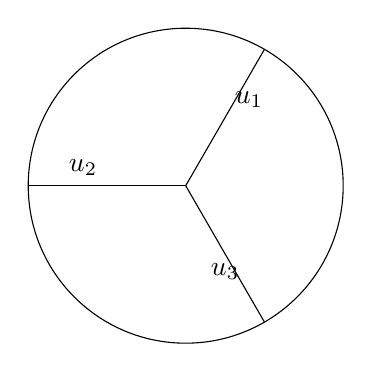
\begin{tikzpicture}
        \draw (0,0) circle (2cm);
        \draw (0,0) -- (60:2cm) node[midway, above right] {$u_1$};
        \draw (0,0) -- (180:2cm) node[midway, above left] {$u_2$};
        \draw (0,0) -- (300:2cm) node[midway, below] {$u_3$};
    \end{tikzpicture}
    \caption{Eğrisel Koordinat Sistemi}
    \label{fig:egrisel_koordinat}
\end{figure}

Bu şema, eğrisel koordinatları $(u_1, u_2, u_3)$ temsil eden bir dairesel gösterim sunar. Bu gösterim, eğrisel koordinatların Kartezyen koordinat sistemi ile ilişkisini anlamak için kullanılabilir.

Eğrisel koordinatlar, belirli bir probleme daha uygun bir koordinat sistemi seçme esnekliği sağlar. Örneğin, silindirik veya küresel koordinatlar, belirli simetrilere sahip problemleri çözmek için daha uygun olabilir.

\subsection{Eğrisel Koordinat Örnekleri}

\subsubsection{Silindirik Koordinatlar $(\rho, \phi, z)$}

Silindirik koordinatlar, üç boyutlu uzayı tanımlamak için kullanılan bir koordinat sistemidir. Bu sistemde, bir noktanın konumu, bir eksene olan uzaklığı $(\rho)$, bu eksen etrafındaki açısı $(\phi)$ ve eksen üzerindeki yüksekliği $(z)$ ile belirlenir.

\textbf{Tanımlar:}

\begin{itemize}
    \item \textit{$\rho$ (rho)}: $xy$ düzlemindeki orijinden olan uzaklık.
    \item \textit{$\phi$ (phi)}: $x$ ekseni ile $\rho$ arasındaki açı (azimut açısı).
    \item \textit{$z$}: $z$ ekseni üzerindeki yükseklik.
\end{itemize}

\textbf{Kartezyen ve Silindirik Koordinatlar Arasındaki İlişki:}

Kartezyen koordinatlardaki $(x, y, z)$ noktası ile silindirik koordinatlardaki $(\rho, \phi, z)$ noktası arasındaki dönüşüm aşağıdaki gibidir:

\begin{itemize}
    \item $x = \rho \cos \phi$
    \item $y = \rho \sin \phi$
    \item $z = z$
\end{itemize}

\textbf{Dönüşümün Tersi:}

\begin{itemize}
    \item $\rho = \sqrt{x^2 + y^2}$
    \item $\phi = \arctan \left( \frac{y}{x} \right)$
    \item $z = z$
\end{itemize}

\textbf{Geometrik Gösterim:}

\begin{figure}[htbp]
    \centering
    \begin{tikzpicture}
        % Eksenleri çiz
        \draw[thick, ->] (-3,0) -- (3,0) node[anchor=north west] {x};
        \draw[thick, ->] (0,-3) -- (0,3) node[anchor=south east] {y};
        \draw[thick, ->] (0,0) -- (1.5,1.5) node[anchor=west] {z};

        % Silindir çiz
        \draw[dashed] (1,0) arc (0:360:1);
        \draw[dashed] (1,0) -- (1,2);
        \draw[dashed] (-1,0) -- (-1,2);
        \draw[dashed] (1,2) arc (0:360:1);

        % P noktası
        \node[circle, fill, inner sep=1.5pt, label=above right:$P$] (P) at (0.7, 1, 1) {};

        % P' noktası
        \node[circle, fill, inner sep=1.5pt, label=below:$P'$] (Pp) at (0.7,0,0) {};

        % rho
        \draw[dashed] (0,0) -- (Pp) node[midway, below] {$\rho$};

        % z
        \draw[dashed] (Pp) -- (P) node[midway, right] {$z$};

        % Açı phi
        \draw (0.4,0) arc (0:45:0.4);
        \node at (0.7,0.3) {$\phi$};

    \end{tikzpicture}
    \caption{Silindirik Koordinat Sistemi}
    \label{fig:silindirik_koordinat}
\end{figure}

Bu şemada:

\begin{itemize}
    \item $P$: Uzaydaki bir noktayı temsil eder.
    \item $P'$: $P$ noktasının $xy$ düzlemindeki izdüşümüdür.
    \item $\rho$: $P'$ noktasının orijine olan uzaklığıdır.
    \item $\phi$: $x$ ekseni ile $OP'$ arasındaki açıdır (azimut açısı).
    \item $z$: $P$ noktasının $z$ ekseni üzerindeki yüksekliğidir.
\end{itemize}

\textbf{Jacobian Dönüşümü:}

Silindirik koordinatlardaki $(\rho, \phi, z)$ ile Kartezyen koordinatlardaki $(x, y, z)$ arasındaki ilişki aşağıdaki gibidir:

\begin{itemize}
    \item $x = \rho \cos \phi$
    \item $y = \rho \sin \phi$
    \item $z = z$
\end{itemize}

Burada $\phi$, azimut açısını temsil etmektedir.

Bu dönüşümü ifade etmek için Jacobian matrisini kullanabiliriz. Jacobian matrisi, koordinat dönüşümünün kısmi türevlerini içerir:

\begin{equation}
J = \begin{bmatrix}
\frac{\partial x}{\partial \rho} & \frac{\partial x}{\partial \phi} & \frac{\partial x}{\partial z} \\
\frac{\partial y}{\partial \rho} & \frac{\partial y}{\partial \phi} & \frac{\partial y}{\partial z} \\
\frac{\partial z}{\partial \rho} & \frac{\partial z}{\partial \phi} & \frac{\partial z}{\partial z}
\end{bmatrix}
\end{equation}

Bu matrisin elemanlarını hesaplarsak:

\begin{itemize}
    \item $\frac{\partial x}{\partial \rho} = \cos \phi$
    \item $\frac{\partial x}{\partial \phi} = -\rho \sin \phi$
    \item $\frac{\partial x}{\partial z} = 0$
    \item $\frac{\partial y}{\partial \rho} = \sin \phi$
    \item $\frac{\partial y}{\partial \phi} = \rho \cos \phi$
    \item $\frac{\partial y}{\partial z} = 0$
    \item $\frac{\partial z}{\partial \rho} = 0$
    \item $\frac{\partial z}{\partial \phi} = 0$
    \item $\frac{\partial z}{\partial z} = 1$
\end{itemize}

Bu değerleri Jacobian matrisine yerleştirdiğimizde:

\begin{equation}
J = \begin{bmatrix}
\cos \phi & -\rho \sin \phi & 0 \\
\sin \phi & \rho \cos \phi & 0 \\
0 & 0 & 1
\end{bmatrix}
\end{equation}

Jacobian determinantı ise şu şekilde hesaplanır:

\begin{equation}
\det(J) = \rho \cos^2 \phi + \rho \sin^2 \phi = \rho (\cos^2 \phi + \sin^2 \phi) = \rho
\end{equation}

Burada $\rho = \sqrt{x^2 + y^2}$ ve $\rho \neq 0$ olmalıdır.

Ayrıca, $\phi = \arctan \left( \frac{y}{x} \right)$ ifadesi kullanılır.

$z = z$ olduğundan, $z$ için türev dönüşümleri basittir.

Bu Jacobian determinantı, hacim elemanının dönüşümünde kullanılır:

\begin{equation}
dV = dx \, dy \, dz = |J| \, d\rho \, d\phi \, dz = \rho \, d\rho \, d\phi \, dz
\end{equation}

Bu dönüşümler, koordinatları bir sistemden diğerine dönüştürmek için kullanılır. Jacobian determinantı, dönüşümün hacim elemanını nasıl etkilediğini gösterir.

\textbf{Silindirik Koordinatların Oluşumu ve Sınır Değerleri}

Silindirik koordinat sistemi, bir levhanın (dikdörtgenin) bir eksen etrafında döndürülmesiyle görselleştirilebilir. Bu bölümde, bu dönüşümün nasıl gerçekleştiğini ve silindirik koordinatların sınır değerlerini inceleyeceğiz.

\textbf{1. Levhanın (Dikdörtgenin) Çizimi:}

İlk olarak, $xz$ düzleminde bir levha (dikdörtgen) çizelim. Bu levha, silindirin yüksekliğini $(z)$ ve yarıçapını $(\rho)$ temsil edecektir.

\begin{figure}[htbp]
    \centering
    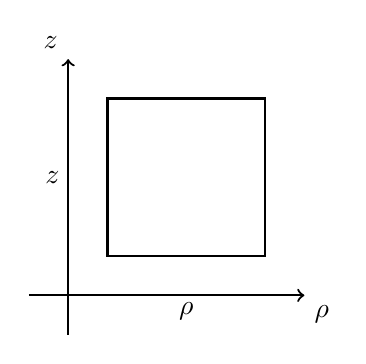
\begin{tikzpicture}
        % Eksenleri çiz
        \draw[thick, ->] (-0.5,0) -- (3,0) node[anchor=north west] {$\rho$};
        \draw[thick, ->] (0,-0.5) -- (0,3) node[anchor=south east] {$z$};

        % Dikdörtgen çiz
        \draw[thick] (0.5,0.5) rectangle (2.5,2.5);
        \node at (1.5, -0.2) {$ \rho $};
        \node at (-0.2, 1.5) {$ z $};
    \end{tikzpicture}
    \caption{$xz$ Düzleminde Dikdörtgen Levha}
    \label{fig:dikdortgen_levha}
\end{figure}

\textbf{2. Döndürme İşlemi:}

Bu levhayı $z$ ekseni etrafında $2\pi$ radyan (360 derece) döndürdüğümüzde, bir silindir elde ederiz. $\phi$ açısı, bu döndürme işlemini temsil eder.

\textbf{3. Silindirin Oluşumu:}

\begin{figure}[htbp]
    \centering
    \begin{tikzpicture}
        % Eksenleri çiz
        \draw[thick, ->] (-3,0) -- (3,0) node[anchor=north west] {x};
        \draw[thick, ->] (0,-3) -- (0,3) node[anchor=south east] {y};
        \draw[thick, ->] (0,0) -- (1.5,1.5) node[anchor=west] {z};

        % Silindir çiz
        \draw[dashed] (1,0) arc (0:360:1);
        \draw[dashed] (1,0) -- (1,2);
        \draw[dashed] (-1,0) -- (-1,2);
        \draw[dashed] (1,2) arc (0:360:1);
    \end{tikzpicture}
    \caption{Silindirik Koordinat Sistemi Oluşumu}
    \label{fig:silindir_olusumu}
\end{figure}

\textbf{4. Sınır Değerleri:}

Silindirik koordinatlarda, her bir değişkenin belirli sınır değerleri vardır:

\begin{itemize}
    \item $\rho$: Yarıçap her zaman pozitif veya sıfır olmalıdır: $\rho \geq 0$.
    \item $\phi$: Azimut açısı genellikle $0$ ile $2\pi$ arasında değişir: $0 \leq \phi < 2\pi$.
    \item $z$: Yükseklik, $-\infty$ ile $+\infty$ arasında herhangi bir değer alabilir: $-\infty < z < +\infty$.
\end{itemize}

\textbf{5. Farklı Döndürme Türleri ve Oluşan Şekiller:}

Eğer levhayı farklı şekillerde döndürürsek, farklı geometrik yapılar elde edebiliriz. Örneğin:

\begin{itemize}
    \item \textbf{Tam Döndürme ($2\pi$)}: $xz$ düzlemindeki dikdörtgenin $z$ ekseni etrafında tam olarak döndürülmesiyle elde edilen silindir.
    \item \textbf{Kısmi Döndürme ($\theta < 2\pi$)}: $xz$ düzlemindeki dikdörtgenin $z$ ekseni etrafında $\theta$ açısı kadar döndürülmesiyle elde edilen silindir parçası.
    \item \textbf{Öteleme}: $xz$ düzlemindeki dikdörtgenin $z$ ekseni boyunca ötelenmesiyle elde edilen prizma.
\end{itemize}

\begin{figure}[htbp]
    \centering
    \begin{tabular}{ccc}
         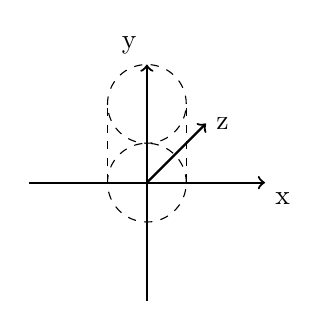
\begin{tikzpicture}[scale=0.5]
        % Eksenleri çiz
        \draw[thick, ->] (-3,0) -- (3,0) node[anchor=north west] {x};
        \draw[thick, ->] (0,-3) -- (0,3) node[anchor=south east] {y};
        \draw[thick, ->] (0,0) -- (1.5,1.5) node[anchor=west] {z};

        % Silindir çiz
        \draw[dashed] (1,0) arc (0:360:1);
        \draw[dashed] (1,0) -- (1,2);
        \draw[dashed] (-1,0) -- (-1,2);
        \draw[dashed] (1,2) arc (0:360:1);
    \end{tikzpicture}
    &
         \begin{tikzpicture}[scale=0.5]
        % Eksenleri çiz
        \draw[thick, ->] (-3,0) -- (3,0) node[anchor=north west] {x};
        \draw[thick, ->] (0,-3) -- (0,3) node[anchor=south east] {y};
        \draw[thick, ->] (0,0) -- (1.5,1.5) node[anchor=west] {z};

        % Silindir çiz
        \draw[dashed] (1,0) arc (0:180:1);
        \draw[dashed] (1,0) -- (1,2);
        \draw[dashed] (-1,0) -- (-1,2);
        \draw[dashed] (1,2) arc (0:180:1);
    \end{tikzpicture}
    &
         \begin{tikzpicture}[scale=0.5]
        % Eksenleri çiz
        \draw[thick, ->] (-3,0) -- (3,0) node[anchor=north west] {x};
        \draw[thick, ->] (0,-3) -- (0,3) node[anchor=south east] {y};
        \draw[thick, ->] (0,0) -- (1.5,1.5) node[anchor=west] {z};

        % Silindir çiz
        \draw[dashed] (1,0) -- (1,2);
        \draw[dashed] (-1,0) -- (-1,2);
        \draw[dashed] (-1,0) -- (1,0);
         \draw[dashed] (-1,2) -- (1,2);
    \end{tikzpicture}
    \\
    Tam Döndürme & Kısmi Döndürme & Öteleme
    \end{tabular}
    \caption{Farklı Döndürme Türleri}
    \label{fig:farkli_dondurme_turleri}
\end{figure}

Bu şemalar, silindirik koordinat sisteminin nasıl oluşturulduğunu ve farklı döndürme türlerinin hangi geometrik yapıları ortaya çıkardığını görsel olarak açıklamaktadır.

\subsubsection{Kutupsal Koordinatlar}

Kutupsal koordinatlar, iki boyutlu uzayı tanımlamak için kullanılan bir koordinat sistemidir. Bu sistemde, bir noktanın konumu, orijine olan uzaklığı $(r)$ ve $x$ ekseni ile yaptığı açı $(\phi)$ ile belirlenir.

\textbf{Kartezyen ve Kutupsal Koordinatlar Arasındaki İlişki:}

Kartezyen koordinatlardaki $(x, y)$ noktası ile kutupsal koordinatlardaki $(r, \phi)$ noktası arasındaki dönüşüm aşağıdaki gibidir:

\begin{itemize}
    \item $x = r \cos \phi$
    \item $y = r \sin \phi$
\end{itemize}

Burada:
\begin{itemize}
    \item $r$: Orijinden olan uzaklık (yarıçap).
    \item $\phi$: $x$ ekseni ile yapılan açı.
\end{itemize}

\textbf{Dönüşümün Tersi:}

\begin{itemize}
    \item $r = \sqrt{x^2 + y^2}$
    \item $\phi = \arctan \left( \frac{y}{x} \right)$
\end{itemize}

\textbf{Jacobian Matrisi:}

\begin{equation}
J = \begin{bmatrix}
\frac{\partial x}{\partial r} & \frac{\partial x}{\partial \phi} \\
\frac{\partial y}{\partial r} & \frac{\partial y}{\partial \phi}
\end{bmatrix} = 
\begin{bmatrix}
\cos \phi & -r \sin \phi \\
\sin \phi & r \cos \phi
\end{bmatrix}
\end{equation}

\begin{equation}
\det(J) = r \cos^2 \phi + r \sin^2 \phi = r \neq 0
\end{equation}

\subsubsection{Küresel Koordinatlar $(r, \theta, \phi)$}

Küresel koordinatlar, üç boyutlu uzayı tanımlamak için kullanılan bir koordinat sistemidir. Bu sistemde, bir noktanın konumu, orijine olan uzaklığı $(r)$, $z$ ekseni ile yaptığı açı $(\theta)$ (zenit açısı veya kutup açısı) ve $x$ ekseni ile $xy$ düzlemindeki izdüşümünün yaptığı açı $(\phi)$ (azimut açısı) ile belirlenir.

\textbf{Tanımlar:}

\begin{itemize}
    \item \textit{$r$}: Orijinden olan uzaklık (yarıçap).
    \item \textit{$\theta$}: $z$ ekseni ile yapılan açı (zenit açısı veya kutup açısı), $0 \leq \theta \leq \pi$.
    \item \textit{$\phi$}: $x$ ekseni ile $xy$ düzlemindeki izdüşümün yaptığı açı (azimut açısı), $0 \leq \phi < 2\pi$.
\end{itemize}

\textbf{Kartezyen ve Küresel Koordinatlar Arasındaki İlişki:}

Kartezyen koordinatlardaki $(x, y, z)$ noktası ile küresel koordinatlardaki $(r, \theta, \phi)$ noktası arasındaki dönüşüm aşağıdaki gibidir:

\begin{itemize}
    \item $x = r \sin \theta \cos \phi$
    \item $y = r \sin \theta \sin \phi$
    \item $z = r \cos \theta$
\end{itemize}

Bu dönüşümlerde:

\begin{itemize}
    \item $x$: Apsis (yatay eksen)
    \item $y$: Ordinat (dikey eksen)
    \item $z$: Kot (derinlik ekseni)
    \item $r$: Orijinden olan uzaklık
    \item $\theta$: Zenit açısı (kutup açısı)
    \item $\phi$: Azimut açısı
\end{itemize}

\end{document}
\documentclass[11pt,letterpaper,twocolumn]{fenbil}
\usepackage{amsmath}
\usepackage{amssymb}
\usepackage{graphicx}
\usepackage{tikz}
\title{FMM - Fizikte Matematiksel Metotlar - Ders Notları}
\author{Celal Ekrem Torun}
\date{6 Mart 2025}

\begin{document}
\twocolumn[\begin{@twocolumnfalse}

\begin{minipage}{0.15\textwidth}{
    }
\end{minipage}
\hspace{25pt}
\begin{minipage}{0.75\textwidth}
\vspace{5mm}
\Large{\textbf{FMM - Fizikte Matematiksel Metotlar - Ders 1 (6 Mart 2025)}}
    \vspace{3mm}
    
    \large{\textbf{Hazırlayan}; Celal Ekrem Torun}
    \vspace{2mm}
    
    \fontsize{0.35cm}{0.5cm}\selectfont \textit{Fizik Bölümü, İstanbul Üniversitesi\newline 
    Beyazıt, Fatih, İstanbul, Türkiye}
    
\end{minipage}

\small

\end{@twocolumnfalse}]

\section{Matematiksel Metotlar}

\textbf{Not:} 1 Mart'ta gradyen vektörü işlendi, 6 Mart'ta eğrisel koordinatlara başlanacak.

\subsection{Gradyen}

\textbf{Tanım:} Bir $\phi(x, y, z)$ skaler alanının gradyeni, o alanın en hızlı değişim yönünü ve büyüklüğünü gösteren bir vektör alanıdır.

Kartezyen koordinatlarda gradyen şu şekilde tanımlanır:

\[
\nabla \phi = \frac{\partial \phi}{\partial x} \hat{e_x} + \frac{\partial \phi}{\partial y} \hat{e_y} + \frac{\partial \phi}{\partial z} \hat{e_z}
\]

Burada:

\begin{itemize}
    \item $\nabla \phi$: Gradyen vektörü
    \item $\phi(x, y, z)$: Skaler alan
    \item $\hat{e_x}$, $\hat{e_y}$, $\hat{e_z}$: Sırasıyla $x$, $y$ ve $z$ yönlerindeki birim vektörler
\end{itemize}

\textbf{Önemli Not:} $\nabla \phi$, $\hat{e_x}$, $\hat{e_y}$ ve $\hat{e_z}$ ile ayrı ayrı skalar çarpılırsa, $\phi$ fonksiyonunun sınırları ile $x$, $y$ ve $z$ doğrultusundaki değişimi bulunur.

Bir $P(x,y,z)$ noktasındaki $\phi$ fonksiyonunun değişim oranı, $\nabla \phi \cdot d\vec{r}$ ile bulunur. Burada $d\vec{r}$, $P$ noktasından küçük bir yer değiştirmeyi temsil eden vektördür. Eğer $\phi = c_1$ yüzeyinden $\phi = c_2$ yüzeyine gidilirse, değişim $d\phi = c_2 - c_1$ olur ve $d\phi \neq 0$ olur.

Eğer $\nabla \phi \cdot d\vec{r} = d\phi = 0$ ise, $\nabla \phi$, $d\vec{r}$ vektörüne diktir. Bu durumda $\nabla \phi$, $\frac{\nabla \phi}{|\nabla \phi|}$ ile aynı yöndedir.

\subsection{Doğrultu Türevi}

\textbf{Tanım:} Bir $\phi(x,y,z)$ skaler alanının, bir $\vec{u}$ birim vektörü yönündeki doğrultu türevi, $\phi$'nin $\vec{u}$ yönündeki değişim oranını verir.

Doğrultu türevi şu şekilde tanımlanır:

\[
\frac{\partial \phi}{\partial u} = \nabla \phi \cdot \hat{u} = |\nabla \phi| |\hat{u}| \cos \theta
\]

Burada:
\begin{itemize}
    \item $\frac{\partial \phi}{\partial u}$: Doğrultu türevi
    \item $\nabla \phi$: Gradyen vektörü
    \item $\hat{u}$: Birim vektör
    \item $\theta$: $\nabla \phi$ ve $\hat{u}$ arasındaki açı
\end{itemize}

$\frac{\partial \phi}{\partial u}$, $\phi$'nin bir $P(x,y,z)$ noktasındaki $\vec{u}$ birim vektörü ile belirlenen doğrultudaki doğrultu türevidir.

$\frac{\partial \phi}{\partial u} = \nabla \phi \cdot \hat{u} = |\nabla \phi| \cos \theta$

\subsection{Örnek Soru}

$\phi(x, y, z) = x^2yz + 4z^2$ fonksiyonunun $P(1, -2, -1)$ noktasındaki $\vec{dr} = (2\hat{e_x} - \hat{e_y} - 2\hat{e_z})$ doğrultusundaki türevini bulun.

\textbf{Çözüm:}

\textit{Adım 1: Gradyeni hesaplayalım:}

$\nabla \phi = (2xyz) \hat{e_x} + (x^2z) \hat{e_y} + (x^2y + 8z) \hat{e_z}$

\textit{Adım 2: P(1, -2, -1) noktasındaki gradyeni hesaplayalım:}

$\nabla \phi |_P = (2(1)(-2)(-1)) \hat{e_x} + ((1)^2(-1)) \hat{e_y} + ((1)^2(-2) + 8(-1)) \hat{e_z} = 4 \hat{e_x} - \hat{e_y} - 10 \hat{e_z}$

\textit{Adım 3: $\vec{u}$ birim vektörünü bulalım:}

$|\vec{dr}| = \sqrt{2^2 + (-1)^2 + (-2)^2} = \sqrt{9} = 3$

$\hat{u} = \frac{\vec{dr}}{|\vec{dr}|} = \frac{2}{3} \hat{e_x} - \frac{1}{3} \hat{e_y} - \frac{2}{3} \hat{e_z}$

\textit{Adım 4: Doğrultu türevini hesaplayalım:}

$\frac{\partial \phi}{\partial u} = \nabla \phi \cdot \hat{u} = (4 \hat{e_x} - \hat{e_y} - 10 \hat{e_z}) \cdot (\frac{2}{3} \hat{e_x} - \frac{1}{3} \hat{e_y} - \frac{2}{3} \hat{e_z}) = \frac{8}{3} + \frac{1}{3} + \frac{20}{3} = \frac{29}{3} \approx 9.67$

\subsection{Eğrisel Koordinatlar}

Üç boyutlu Öklit uzayında, bir noktanın Kartezyen koordinatları $(x, y, z)$ ile ifade edilir. Şimdi, bu koordinatlara bağlı üç yeni değişken tanımlayalım:

\begin{equation}
u_1 = u_1(x, y, z)
\end{equation}
\begin{equation}
u_2 = u_2(x, y, z)
\end{equation}
\begin{equation}
u_3 = u_3(x, y, z)
\end{equation}

Bu yeni değişkenler, eğrisel koordinatları temsil eder.

\subsubsection{$u_1$, $u_2$, $u_3$'ün Bağımsız Fonksiyonlar Olması}

Lineer homojen bir sistemin sıfırdan farklı çözüme sahip olabilmesi için, katsayılar determinantının sıfıra eşit olması gerekmektedir. Şimdi, $u_1$, $u_2$, $u_3$'ün bağımsız fonksiyonlar olmasının ne anlama geldiğini inceleyelim.

$u_1(x, y, z)$, $u_2(x, y, z)$ ve $u_3(x, y, z)$ fonksiyonları için aşağıdaki ifadeler tanımlanır:

\begin{equation}
u_1 = u_1(x, y, z)
\end{equation}
\begin{equation}
u_2 = u_2(x, y, z)
\end{equation}
\begin{equation}
u_3 = u_3(x, y, z)
\end{equation}

Bu fonksiyonların diferansiyelleri ise şu şekildedir:

\begin{equation}
du_1 = \frac{\partial u_1}{\partial x} dx + \frac{\partial u_1}{\partial y} dy + \frac{\partial u_1}{\partial z} dz
\end{equation}
\begin{equation}
du_2 = \frac{\partial u_2}{\partial x} dx + \frac{\partial u_2}{\partial y} dy + \frac{\partial u_2}{\partial z} dz
\end{equation}
\begin{equation}
du_3 = \frac{\partial u_3}{\partial x} dx + \frac{\partial u_3}{\partial y} dy + \frac{\partial u_3}{\partial z} dz
\end{equation}

Bu denklemleri matris formunda ifade edebiliriz:

\begin{equation}
\begin{bmatrix} du_1 \\ du_2 \\ du_3 \end{bmatrix} = 
\begin{bmatrix}
\frac{\partial u_1}{\partial x} & \frac{\partial u_1}{\partial y} & \frac{\partial u_1}{\partial z} \\
\frac{\partial u_2}{\partial x} & \frac{\partial u_2}{\partial y} & \frac{\partial u_2}{\partial z} \\
\frac{\partial u_3}{\partial x} & \frac{\partial u_3}{\partial y} & \frac{\partial u_3}{\partial z}
\end{bmatrix}
\begin{bmatrix} dx \\ dy \\ dz \end{bmatrix}
\end{equation}

Bu matrisi daha kompakt bir şekilde ifade etmek için, aşağıdaki tanımlamaları yapalım:

\begin{equation}
d\mathbf{u} = \begin{bmatrix} du_1 \\ du_2 \\ du_3 \end{bmatrix}, \quad
A = \begin{bmatrix}
\frac{\partial u_1}{\partial x} & \frac{\partial u_1}{\partial y} & \frac{\partial u_1}{\partial z} \\
\frac{\partial u_2}{\partial x} & \frac{\partial u_2}{\partial y} & \frac{\partial u_2}{\partial z} \\
\frac{\partial u_3}{\partial x} & \frac{\partial u_3}{\partial y} & \frac{\partial u_3}{\partial z}
\end{bmatrix}, \quad
d\mathbf{x} = \begin{bmatrix} dx \\ dy \\ dz \end{bmatrix}
\end{equation}

Bu durumda, yukarıdaki denklem şu şekilde yazılabilir:

\begin{equation}
d\mathbf{u} = A \, d\mathbf{x}
\end{equation}

$dx$, $dy$ ve $dz$'yi $du_1$, $du_2$ ve $du_3$ cinsinden ifade etmek için, $A$ matrisinin tersini almamız gerekir:

\begin{equation}
d\mathbf{x} = A^{-1} \, d\mathbf{u}
\end{equation}

$A^{-1}$ matrisinin var olabilmesi için, $A$ matrisinin determinantı sıfırdan farklı olmalıdır:

\begin{equation}
J = \det(A) \neq 0
\end{equation}

Burada $J$, Jacobian determinantıdır. $A^{-1}$ matrisi, $A$'nın ek matrisinin determinantına bölünmesiyle bulunur:

\begin{equation}
A^{-1} = \frac{\text{adj}(A)}{J}
\end{equation}

Bu durumda, $dx$, $dy$ ve $dz$ aşağıdaki şekilde ifade edilebilir:

\begin{equation}
\begin{bmatrix} dx \\ dy \\ dz \end{bmatrix} = A^{-1} \begin{bmatrix} du_1 \\ du_2 \\ du_3 \end{bmatrix}
\end{equation}

Kartezyen koordinatları eğrisel koordinatlar cinsinden ifade etmek için, aşağıdaki bağıntıları kullanırız:

\begin{equation}
x = x(u_1, u_2, u_3)
\end{equation}
\begin{equation}
y = y(u_1, u_2, u_3)
\end{equation}
\begin{equation}
z = z(u_1, u_2, u_3)
\end{equation}

Bu durumda, konum vektörü $\vec{r}$ aşağıdaki gibi ifade edilir:

\begin{equation}
\vec{r} = x(u_1, u_2, u_3) \, \hat{e_x} + y(u_1, u_2, u_3) \, \hat{e_y} + z(u_1, u_2, u_3) \, \hat{e_z}
\end{equation}

\subsubsection{Eğrisel Koordinatların Geometrik Gösterimi}

Aşağıdaki şemalar, eğrisel koordinatların ve Kartezyen koordinat sisteminin ayrı ayrı gösterimlerini sunmaktadır.

\textbf{Kartezyen Koordinat Sistemi:}

\begin{figure}[htbp]
    \centering
    \begin{tikzpicture}
        \draw[thick, ->] (-3,0) -- (3,0) node[anchor=north west] {x};
        \draw[thick, ->] (0,-3) -- (0,3) node[anchor=south east] {y};
        \draw[thick, ->] (0,0) -- (1.5,1.5) node[anchor=west] {z};
        
        \node[below right] at (2.2, -0.2) {Apsis (x)};
        \node[above] at (-2.2, 0) {Ordinat (y)};
    \end{tikzpicture}
    \caption{Kartezyen Koordinat Sistemi}
    \label{fig:kartezyen_koordinat}
\end{figure}

Bu şemada:

\begin{itemize}
    \item \textit{Apsis (x)}: Yatay ekseni temsil eder.
    \item \textit{Ordinat (y)}: Dikey ekseni temsil eder.
    \item \textit{Kot (z)}: Derinlik eksenini temsil eder.
\end{itemize}

\textbf{Eğrisel Koordinat Sistemi Gösterimi:}

\begin{figure}[htbp]
    \centering
    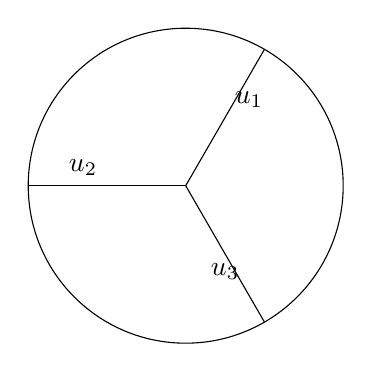
\begin{tikzpicture}
        \draw (0,0) circle (2cm);
        \draw (0,0) -- (60:2cm) node[midway, above right] {$u_1$};
        \draw (0,0) -- (180:2cm) node[midway, above left] {$u_2$};
        \draw (0,0) -- (300:2cm) node[midway, below] {$u_3$};
    \end{tikzpicture}
    \caption{Eğrisel Koordinat Sistemi}
    \label{fig:egrisel_koordinat}
\end{figure}

Bu şema, eğrisel koordinatları $(u_1, u_2, u_3)$ temsil eden bir dairesel gösterim sunar. Bu gösterim, eğrisel koordinatların Kartezyen koordinat sistemi ile ilişkisini anlamak için kullanılabilir.

Eğrisel koordinatlar, belirli bir probleme daha uygun bir koordinat sistemi seçme esnekliği sağlar. Örneğin, silindirik veya küresel koordinatlar, belirli simetrilere sahip problemleri çözmek için daha uygun olabilir.

\subsection{Eğrisel Koordinat Örnekleri}

\subsubsection{Silindirik Koordinatlar $(\rho, \phi, z)$}

Silindirik koordinatlar, üç boyutlu uzayı tanımlamak için kullanılan bir koordinat sistemidir. Bu sistemde, bir noktanın konumu, bir eksene olan uzaklığı $(\rho)$, bu eksen etrafındaki açısı $(\phi)$ ve eksen üzerindeki yüksekliği $(z)$ ile belirlenir.

\textbf{Tanımlar:}

\begin{itemize}
    \item \textit{$\rho$ (rho)}: $xy$ düzlemindeki orijinden olan uzaklık.
    \item \textit{$\phi$ (phi)}: $x$ ekseni ile $\rho$ arasındaki açı (azimut açısı).
    \item \textit{$z$}: $z$ ekseni üzerindeki yükseklik.
\end{itemize}

\textbf{Kartezyen ve Silindirik Koordinatlar Arasındaki İlişki:}

Kartezyen koordinatlardaki $(x, y, z)$ noktası ile silindirik koordinatlardaki $(\rho, \phi, z)$ noktası arasındaki dönüşüm aşağıdaki gibidir:

\begin{itemize}
    \item $x = \rho \cos \phi$
    \item $y = \rho \sin \phi$
    \item $z = z$
\end{itemize}

\textbf{Dönüşümün Tersi:}

\begin{itemize}
    \item $\rho = \sqrt{x^2 + y^2}$
    \item $\phi = \arctan \left( \frac{y}{x} \right)$
    \item $z = z$
\end{itemize}

\textbf{Geometrik Gösterim:}

\begin{figure}[htbp]
    \centering
    \begin{tikzpicture}
        % Eksenleri çiz
        \draw[thick, ->] (-3,0) -- (3,0) node[anchor=north west] {x};
        \draw[thick, ->] (0,-3) -- (0,3) node[anchor=south east] {y};
        \draw[thick, ->] (0,0) -- (1.5,1.5) node[anchor=west] {z};

        % Silindir çiz
        \draw[dashed] (1,0) arc (0:360:1);
        \draw[dashed] (1,0) -- (1,2);
        \draw[dashed] (-1,0) -- (-1,2);
        \draw[dashed] (1,2) arc (0:360:1);

        % P noktası
        \node[circle, fill, inner sep=1.5pt, label=above right:$P$] (P) at (0.7, 1, 1) {};

        % P' noktası
        \node[circle, fill, inner sep=1.5pt, label=below:$P'$] (Pp) at (0.7,0,0) {};

        % rho
        \draw[dashed] (0,0) -- (Pp) node[midway, below] {$\rho$};

        % z
        \draw[dashed] (Pp) -- (P) node[midway, right] {$z$};

        % Açı phi
        \draw (0.4,0) arc (0:45:0.4);
        \node at (0.7,0.3) {$\phi$};

    \end{tikzpicture}
    \caption{Silindirik Koordinat Sistemi}
    \label{fig:silindirik_koordinat}
\end{figure}

Bu şemada:

\begin{itemize}
    \item $P$: Uzaydaki bir noktayı temsil eder.
    \item $P'$: $P$ noktasının $xy$ düzlemindeki izdüşümüdür.
    \item $\rho$: $P'$ noktasının orijine olan uzaklığıdır.
    \item $\phi$: $x$ ekseni ile $OP'$ arasındaki açıdır (azimut açısı).
    \item $z$: $P$ noktasının $z$ ekseni üzerindeki yüksekliğidir.
\end{itemize}

\textbf{Jacobian Dönüşümü:}

Silindirik koordinatlardaki $(\rho, \phi, z)$ ile Kartezyen koordinatlardaki $(x, y, z)$ arasındaki ilişki aşağıdaki gibidir:

\begin{itemize}
    \item $x = \rho \cos \phi$
    \item $y = \rho \sin \phi$
    \item $z = z$
\end{itemize}

Burada $\phi$, azimut açısını temsil etmektedir.

Bu dönüşümü ifade etmek için Jacobian matrisini kullanabiliriz. Jacobian matrisi, koordinat dönüşümünün kısmi türevlerini içerir:

\begin{equation}
J = \begin{bmatrix}
\frac{\partial x}{\partial \rho} & \frac{\partial x}{\partial \phi} & \frac{\partial x}{\partial z} \\
\frac{\partial y}{\partial \rho} & \frac{\partial y}{\partial \phi} & \frac{\partial y}{\partial z} \\
\frac{\partial z}{\partial \rho} & \frac{\partial z}{\partial \phi} & \frac{\partial z}{\partial z}
\end{bmatrix}
\end{equation}

Bu matrisin elemanlarını hesaplarsak:

\begin{itemize}
    \item $\frac{\partial x}{\partial \rho} = \cos \phi$
    \item $\frac{\partial x}{\partial \phi} = -\rho \sin \phi$
    \item $\frac{\partial x}{\partial z} = 0$
    \item $\frac{\partial y}{\partial \rho} = \sin \phi$
    \item $\frac{\partial y}{\partial \phi} = \rho \cos \phi$
    \item $\frac{\partial y}{\partial z} = 0$
    \item $\frac{\partial z}{\partial \rho} = 0$
    \item $\frac{\partial z}{\partial \phi} = 0$
    \item $\frac{\partial z}{\partial z} = 1$
\end{itemize}

Bu değerleri Jacobian matrisine yerleştirdiğimizde:

\begin{equation}
J = \begin{bmatrix}
\cos \phi & -\rho \sin \phi & 0 \\
\sin \phi & \rho \cos \phi & 0 \\
0 & 0 & 1
\end{bmatrix}
\end{equation}

Jacobian determinantı ise şu şekilde hesaplanır:

\begin{equation}
\det(J) = \rho \cos^2 \phi + \rho \sin^2 \phi = \rho (\cos^2 \phi + \sin^2 \phi) = \rho
\end{equation}

Burada $\rho = \sqrt{x^2 + y^2}$ ve $\rho \neq 0$ olmalıdır.

Ayrıca, $\phi = \arctan \left( \frac{y}{x} \right)$ ifadesi kullanılır.

$z = z$ olduğundan, $z$ için türev dönüşümleri basittir.

Bu Jacobian determinantı, hacim elemanının dönüşümünde kullanılır:

\begin{equation}
dV = dx \, dy \, dz = |J| \, d\rho \, d\phi \, dz = \rho \, d\rho \, d\phi \, dz
\end{equation}

Bu dönüşümler, koordinatları bir sistemden diğerine dönüştürmek için kullanılır. Jacobian determinantı, dönüşümün hacim elemanını nasıl etkilediğini gösterir.

\textbf{Silindirik Koordinatların Oluşumu ve Sınır Değerleri}

Silindirik koordinat sistemi, bir levhanın (dikdörtgenin) bir eksen etrafında döndürülmesiyle görselleştirilebilir. Bu bölümde, bu dönüşümün nasıl gerçekleştiğini ve silindirik koordinatların sınır değerlerini inceleyeceğiz.

\textbf{1. Levhanın (Dikdörtgenin) Çizimi:}

İlk olarak, $xz$ düzleminde bir levha (dikdörtgen) çizelim. Bu levha, silindirin yüksekliğini $(z)$ ve yarıçapını $(\rho)$ temsil edecektir.

\begin{figure}[htbp]
    \centering
    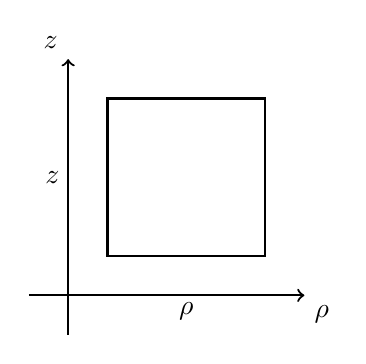
\begin{tikzpicture}
        % Eksenleri çiz
        \draw[thick, ->] (-0.5,0) -- (3,0) node[anchor=north west] {$\rho$};
        \draw[thick, ->] (0,-0.5) -- (0,3) node[anchor=south east] {$z$};

        % Dikdörtgen çiz
        \draw[thick] (0.5,0.5) rectangle (2.5,2.5);
        \node at (1.5, -0.2) {$ \rho $};
        \node at (-0.2, 1.5) {$ z $};
    \end{tikzpicture}
    \caption{$xz$ Düzleminde Dikdörtgen Levha}
    \label{fig:dikdortgen_levha}
\end{figure}

\textbf{2. Döndürme İşlemi:}

Bu levhayı $z$ ekseni etrafında $2\pi$ radyan (360 derece) döndürdüğümüzde, bir silindir elde ederiz. $\phi$ açısı, bu döndürme işlemini temsil eder.

\textbf{3. Silindirin Oluşumu:}

\begin{figure}[htbp]
    \centering
    \begin{tikzpicture}
        % Eksenleri çiz
        \draw[thick, ->] (-3,0) -- (3,0) node[anchor=north west] {x};
        \draw[thick, ->] (0,-3) -- (0,3) node[anchor=south east] {y};
        \draw[thick, ->] (0,0) -- (1.5,1.5) node[anchor=west] {z};

        % Silindir çiz
        \draw[dashed] (1,0) arc (0:360:1);
        \draw[dashed] (1,0) -- (1,2);
        \draw[dashed] (-1,0) -- (-1,2);
        \draw[dashed] (1,2) arc (0:360:1);
    \end{tikzpicture}
    \caption{Silindirik Koordinat Sistemi Oluşumu}
    \label{fig:silindir_olusumu}
\end{figure}

\textbf{4. Sınır Değerleri:}

Silindirik koordinatlarda, her bir değişkenin belirli sınır değerleri vardır:

\begin{itemize}
    \item $\rho$: Yarıçap her zaman pozitif veya sıfır olmalıdır: $\rho \geq 0$.
    \item $\phi$: Azimut açısı genellikle $0$ ile $2\pi$ arasında değişir: $0 \leq \phi < 2\pi$.
    \item $z$: Yükseklik, $-\infty$ ile $+\infty$ arasında herhangi bir değer alabilir: $-\infty < z < +\infty$.
\end{itemize}

\textbf{5. Farklı Döndürme Türleri ve Oluşan Şekiller:}

Eğer levhayı farklı şekillerde döndürürsek, farklı geometrik yapılar elde edebiliriz. Örneğin:

\begin{itemize}
    \item \textbf{Tam Döndürme ($2\pi$)}: $xz$ düzlemindeki dikdörtgenin $z$ ekseni etrafında tam olarak döndürülmesiyle elde edilen silindir.
    \item \textbf{Kısmi Döndürme ($\theta < 2\pi$)}: $xz$ düzlemindeki dikdörtgenin $z$ ekseni etrafında $\theta$ açısı kadar döndürülmesiyle elde edilen silindir parçası.
    \item \textbf{Öteleme}: $xz$ düzlemindeki dikdörtgenin $z$ ekseni boyunca ötelenmesiyle elde edilen prizma.
\end{itemize}

\begin{figure}[htbp]
    \centering
    \begin{tabular}{ccc}
         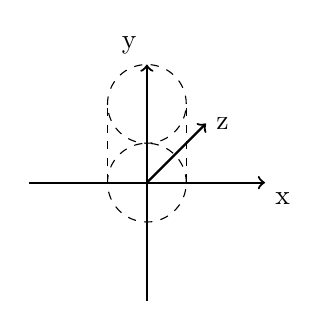
\begin{tikzpicture}[scale=0.5]
        % Eksenleri çiz
        \draw[thick, ->] (-3,0) -- (3,0) node[anchor=north west] {x};
        \draw[thick, ->] (0,-3) -- (0,3) node[anchor=south east] {y};
        \draw[thick, ->] (0,0) -- (1.5,1.5) node[anchor=west] {z};

        % Silindir çiz
        \draw[dashed] (1,0) arc (0:360:1);
        \draw[dashed] (1,0) -- (1,2);
        \draw[dashed] (-1,0) -- (-1,2);
        \draw[dashed] (1,2) arc (0:360:1);
    \end{tikzpicture}
    &
         \begin{tikzpicture}[scale=0.5]
        % Eksenleri çiz
        \draw[thick, ->] (-3,0) -- (3,0) node[anchor=north west] {x};
        \draw[thick, ->] (0,-3) -- (0,3) node[anchor=south east] {y};
        \draw[thick, ->] (0,0) -- (1.5,1.5) node[anchor=west] {z};

        % Silindir çiz
        \draw[dashed] (1,0) arc (0:180:1);
        \draw[dashed] (1,0) -- (1,2);
        \draw[dashed] (-1,0) -- (-1,2);
        \draw[dashed] (1,2) arc (0:180:1);
    \end{tikzpicture}
    &
         \begin{tikzpicture}[scale=0.5]
        % Eksenleri çiz
        \draw[thick, ->] (-3,0) -- (3,0) node[anchor=north west] {x};
        \draw[thick, ->] (0,-3) -- (0,3) node[anchor=south east] {y};
        \draw[thick, ->] (0,0) -- (1.5,1.5) node[anchor=west] {z};

        % Silindir çiz
        \draw[dashed] (1,0) -- (1,2);
        \draw[dashed] (-1,0) -- (-1,2);
        \draw[dashed] (-1,0) -- (1,0);
         \draw[dashed] (-1,2) -- (1,2);
    \end{tikzpicture}
    \\
    Tam Döndürme & Kısmi Döndürme & Öteleme
    \end{tabular}
    \caption{Farklı Döndürme Türleri}
    \label{fig:farkli_dondurme_turleri}
\end{figure}

Bu şemalar, silindirik koordinat sisteminin nasıl oluşturulduğunu ve farklı döndürme türlerinin hangi geometrik yapıları ortaya çıkardığını görsel olarak açıklamaktadır.

\end{document}
\documentclass[11pt,letterpaper,twocolumn]{fenbil}
\usepackage{amsmath}
\usepackage{amssymb}
\usepackage{graphicx}
\usepackage{tikz}
\title{FMM - Fizikte Matematiksel Metotlar - Ders Notları}
\author{Celal Ekrem Torun}
\date{6 Mart 2025}

\begin{document}
\twocolumn[\begin{@twocolumnfalse}

\begin{minipage}{0.15\textwidth}{
    }
\end{minipage}
\hspace{25pt}
\begin{minipage}{0.75\textwidth}
\vspace{5mm}
\Large{\textbf{FMM - Fizikte Matematiksel Metotlar - Ders 1 (6 Mart 2025)}}
    \vspace{3mm}
    
    \large{\textbf{Hazırlayan}; Celal Ekrem Torun}
    \vspace{2mm}
    
    \fontsize{0.35cm}{0.5cm}\selectfont \textit{Fizik Bölümü, İstanbul Üniversitesi\newline 
    Beyazıt, Fatih, İstanbul, Türkiye}
    
\end{minipage}

\small

\end{@twocolumnfalse}]

\section{Matematiksel Metotlar}

\textbf{Not:} 1 Mart'ta gradyen vektörü işlendi, 6 Mart'ta eğrisel koordinatlara başlanacak.

\subsection{Gradyen}

\textbf{Tanım:} Bir $\phi(x, y, z)$ skaler alanının gradyeni, o alanın en hızlı değişim yönünü ve büyüklüğünü gösteren bir vektör alanıdır.

Kartezyen koordinatlarda gradyen şu şekilde tanımlanır:

\[
\nabla \phi = \frac{\partial \phi}{\partial x} \hat{e_x} + \frac{\partial \phi}{\partial y} \hat{e_y} + \frac{\partial \phi}{\partial z} \hat{e_z}
\]

Burada:

\begin{itemize}
    \item $\nabla \phi$: Gradyen vektörü
    \item $\phi(x, y, z)$: Skaler alan
    \item $\hat{e_x}$, $\hat{e_y}$, $\hat{e_z}$: Sırasıyla $x$, $y$ ve $z$ yönlerindeki birim vektörler
\end{itemize}

\textbf{Önemli Not:} $\nabla \phi$, $\hat{e_x}$, $\hat{e_y}$ ve $\hat{e_z}$ ile ayrı ayrı skalar çarpılırsa, $\phi$ fonksiyonunun sınırları ile $x$, $y$ ve $z$ doğrultusundaki değişimi bulunur.

Bir $P(x,y,z)$ noktasındaki $\phi$ fonksiyonunun değişim oranı, $\nabla \phi \cdot d\vec{r}$ ile bulunur. Burada $d\vec{r}$, $P$ noktasından küçük bir yer değiştirmeyi temsil eden vektördür. Eğer $\phi = c_1$ yüzeyinden $\phi = c_2$ yüzeyine gidilirse, değişim $d\phi = c_2 - c_1$ olur ve $d\phi \neq 0$ olur.

Eğer $\nabla \phi \cdot d\vec{r} = d\phi = 0$ ise, $\nabla \phi$, $d\vec{r}$ vektörüne diktir. Bu durumda $\nabla \phi$, $\frac{\nabla \phi}{|\nabla \phi|}$ ile aynı yöndedir.

\subsection{Doğrultu Türevi}

\textbf{Tanım:} Bir $\phi(x,y,z)$ skaler alanının, bir $\vec{u}$ birim vektörü yönündeki doğrultu türevi, $\phi$'nin $\vec{u}$ yönündeki değişim oranını verir.

Doğrultu türevi şu şekilde tanımlanır:

\[
\frac{\partial \phi}{\partial u} = \nabla \phi \cdot \hat{u} = |\nabla \phi| |\hat{u}| \cos \theta
\]

Burada:
\begin{itemize}
    \item $\frac{\partial \phi}{\partial u}$: Doğrultu türevi
    \item $\nabla \phi$: Gradyen vektörü
    \item $\hat{u}$: Birim vektör
    \item $\theta$: $\nabla \phi$ ve $\hat{u}$ arasındaki açı
\end{itemize}

$\frac{\partial \phi}{\partial u}$, $\phi$'nin bir $P(x,y,z)$ noktasındaki $\vec{u}$ birim vektörü ile belirlenen doğrultudaki doğrultu türevidir.

$\frac{\partial \phi}{\partial u} = \nabla \phi \cdot \hat{u} = |\nabla \phi| \cos \theta$

\subsection{Örnek Soru}

$\phi(x, y, z) = x^2yz + 4z^2$ fonksiyonunun $P(1, -2, -1)$ noktasındaki $\vec{dr} = (2\hat{e_x} - \hat{e_y} - 2\hat{e_z})$ doğrultusundaki türevini bulun.

\textbf{Çözüm:}

\textit{Adım 1: Gradyeni hesaplayalım:}

$\nabla \phi = (2xyz) \hat{e_x} + (x^2z) \hat{e_y} + (x^2y + 8z) \hat{e_z}$

\textit{Adım 2: P(1, -2, -1) noktasındaki gradyeni hesaplayalım:}

$\nabla \phi |_P = (2(1)(-2)(-1)) \hat{e_x} + ((1)^2(-1)) \hat{e_y} + ((1)^2(-2) + 8(-1)) \hat{e_z} = 4 \hat{e_x} - \hat{e_y} - 10 \hat{e_z}$

\textit{Adım 3: $\vec{u}$ birim vektörünü bulalım:}

$|\vec{dr}| = \sqrt{2^2 + (-1)^2 + (-2)^2} = \sqrt{9} = 3$

$\hat{u} = \frac{\vec{dr}}{|\vec{dr}|} = \frac{2}{3} \hat{e_x} - \frac{1}{3} \hat{e_y} - \frac{2}{3} \hat{e_z}$

\textit{Adım 4: Doğrultu türevini hesaplayalım:}

$\frac{\partial \phi}{\partial u} = \nabla \phi \cdot \hat{u} = (4 \hat{e_x} - \hat{e_y} - 10 \hat{e_z}) \cdot (\frac{2}{3} \hat{e_x} - \frac{1}{3} \hat{e_y} - \frac{2}{3} \hat{e_z}) = \frac{8}{3} + \frac{1}{3} + \frac{20}{3} = \frac{29}{3} \approx 9.67$

\subsection{Eğrisel Koordinatlar}

Üç boyutlu Öklit uzayında, bir noktanın Kartezyen koordinatları $(x, y, z)$ ile ifade edilir. Şimdi, bu koordinatlara bağlı üç yeni değişken tanımlayalım:

\begin{equation}
u_1 = u_1(x, y, z)
\end{equation}
\begin{equation}
u_2 = u_2(x, y, z)
\end{equation}
\begin{equation}
u_3 = u_3(x, y, z)
\end{equation}

Bu yeni değişkenler, eğrisel koordinatları temsil eder.

\subsubsection{$u_1$, $u_2$, $u_3$'ün Bağımsız Fonksiyonlar Olması}

Lineer homojen bir sistemin sıfırdan farklı çözüme sahip olabilmesi için, katsayılar determinantının sıfıra eşit olması gerekmektedir. Şimdi, $u_1$, $u_2$, $u_3$'ün bağımsız fonksiyonlar olmasının ne anlama geldiğini inceleyelim.

$u_1(x, y, z)$, $u_2(x, y, z)$ ve $u_3(x, y, z)$ fonksiyonları için aşağıdaki ifadeler tanımlanır:

\begin{equation}
u_1 = u_1(x, y, z)
\end{equation}
\begin{equation}
u_2 = u_2(x, y, z)
\end{equation}
\begin{equation}
u_3 = u_3(x, y, z)
\end{equation}

Bu fonksiyonların diferansiyelleri ise şu şekildedir:

\begin{equation}
du_1 = \frac{\partial u_1}{\partial x} dx + \frac{\partial u_1}{\partial y} dy + \frac{\partial u_1}{\partial z} dz
\end{equation}
\begin{equation}
du_2 = \frac{\partial u_2}{\partial x} dx + \frac{\partial u_2}{\partial y} dy + \frac{\partial u_2}{\partial z} dz
\end{equation}
\begin{equation}
du_3 = \frac{\partial u_3}{\partial x} dx + \frac{\partial u_3}{\partial y} dy + \frac{\partial u_3}{\partial z} dz
\end{equation}

Bu denklemleri matris formunda ifade edebiliriz:

\begin{equation}
\begin{bmatrix} du_1 \\ du_2 \\ du_3 \end{bmatrix} = 
\begin{bmatrix}
\frac{\partial u_1}{\partial x} & \frac{\partial u_1}{\partial y} & \frac{\partial u_1}{\partial z} \\
\frac{\partial u_2}{\partial x} & \frac{\partial u_2}{\partial y} & \frac{\partial u_2}{\partial z} \\
\frac{\partial u_3}{\partial x} & \frac{\partial u_3}{\partial y} & \frac{\partial u_3}{\partial z}
\end{bmatrix}
\begin{bmatrix} dx \\ dy \\ dz \end{bmatrix}
\end{equation}

Bu matrisi daha kompakt bir şekilde ifade etmek için, aşağıdaki tanımlamaları yapalım:

\begin{equation}
d\mathbf{u} = \begin{bmatrix} du_1 \\ du_2 \\ du_3 \end{bmatrix}, \quad
A = \begin{bmatrix}
\frac{\partial u_1}{\partial x} & \frac{\partial u_1}{\partial y} & \frac{\partial u_1}{\partial z} \\
\frac{\partial u_2}{\partial x} & \frac{\partial u_2}{\partial y} & \frac{\partial u_2}{\partial z} \\
\frac{\partial u_3}{\partial x} & \frac{\partial u_3}{\partial y} & \frac{\partial u_3}{\partial z}
\end{bmatrix}, \quad
d\mathbf{x} = \begin{bmatrix} dx \\ dy \\ dz \end{bmatrix}
\end{equation}

Bu durumda, yukarıdaki denklem şu şekilde yazılabilir:

\begin{equation}
d\mathbf{u} = A \, d\mathbf{x}
\end{equation}

$dx$, $dy$ ve $dz$'yi $du_1$, $du_2$ ve $du_3$ cinsinden ifade etmek için, $A$ matrisinin tersini almamız gerekir:

\begin{equation}
d\mathbf{x} = A^{-1} \, d\mathbf{u}
\end{equation}

$A^{-1}$ matrisinin var olabilmesi için, $A$ matrisinin determinantı sıfırdan farklı olmalıdır:

\begin{equation}
J = \det(A) \neq 0
\end{equation}

Burada $J$, Jacobian determinantıdır. $A^{-1}$ matrisi, $A$'nın ek matrisinin determinantına bölünmesiyle bulunur:

\begin{equation}
A^{-1} = \frac{\text{adj}(A)}{J}
\end{equation}

Bu durumda, $dx$, $dy$ ve $dz$ aşağıdaki şekilde ifade edilebilir:

\begin{equation}
\begin{bmatrix} dx \\ dy \\ dz \end{bmatrix} = A^{-1} \begin{bmatrix} du_1 \\ du_2 \\ du_3 \end{bmatrix}
\end{equation}

Kartezyen koordinatları eğrisel koordinatlar cinsinden ifade etmek için, aşağıdaki bağıntıları kullanırız:

\begin{equation}
x = x(u_1, u_2, u_3)
\end{equation}
\begin{equation}
y = y(u_1, u_2, u_3)
\end{equation}
\begin{equation}
z = z(u_1, u_2, u_3)
\end{equation}

Bu durumda, konum vektörü $\vec{r}$ aşağıdaki gibi ifade edilir:

\begin{equation}
\vec{r} = x(u_1, u_2, u_3) \, \hat{e_x} + y(u_1, u_2, u_3) \, \hat{e_y} + z(u_1, u_2, u_3) \, \hat{e_z}
\end{equation}

\subsubsection{Eğrisel Koordinatların Geometrik Gösterimi}

Aşağıdaki şemalar, eğrisel koordinatların ve Kartezyen koordinat sisteminin ayrı ayrı gösterimlerini sunmaktadır.

\textbf{Kartezyen Koordinat Sistemi:}

\begin{figure}[htbp]
    \centering
    \begin{tikzpicture}
        \draw[thick, ->] (-3,0) -- (3,0) node[anchor=north west] {x};
        \draw[thick, ->] (0,-3) -- (0,3) node[anchor=south east] {y};
        \draw[thick, ->] (0,0) -- (1.5,1.5) node[anchor=west] {z};
        
        \node[below right] at (2.2, -0.2) {Apsis (x)};
        \node[above] at (-2.2, 0) {Ordinat (y)};
    \end{tikzpicture}
    \caption{Kartezyen Koordinat Sistemi}
    \label{fig:kartezyen_koordinat}
\end{figure}

Bu şemada:

\begin{itemize}
    \item \textit{Apsis (x)}: Yatay ekseni temsil eder.
    \item \textit{Ordinat (y)}: Dikey ekseni temsil eder.
    \item \textit{Kot (z)}: Derinlik eksenini temsil eder.
\end{itemize}

\textbf{Eğrisel Koordinat Sistemi Gösterimi:}

\begin{figure}[htbp]
    \centering
    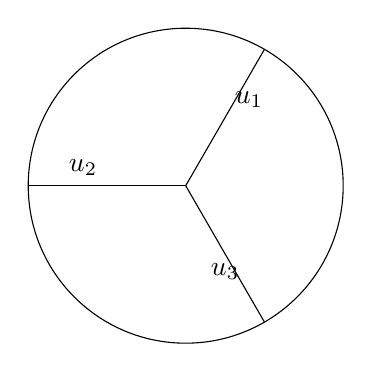
\begin{tikzpicture}
        \draw (0,0) circle (2cm);
        \draw (0,0) -- (60:2cm) node[midway, above right] {$u_1$};
        \draw (0,0) -- (180:2cm) node[midway, above left] {$u_2$};
        \draw (0,0) -- (300:2cm) node[midway, below] {$u_3$};
    \end{tikzpicture}
    \caption{Eğrisel Koordinat Sistemi}
    \label{fig:egrisel_koordinat}
\end{figure}

Bu şema, eğrisel koordinatları $(u_1, u_2, u_3)$ temsil eden bir dairesel gösterim sunar. Bu gösterim, eğrisel koordinatların Kartezyen koordinat sistemi ile ilişkisini anlamak için kullanılabilir.

Eğrisel koordinatlar, belirli bir probleme daha uygun bir koordinat sistemi seçme esnekliği sağlar. Örneğin, silindirik veya küresel koordinatlar, belirli simetrilere sahip problemleri çözmek için daha uygun olabilir.

\subsection{Eğrisel Koordinat Örnekleri}

\subsubsection{Silindirik Koordinatlar $(\rho, \phi, z)$}

Silindirik koordinatlar, üç boyutlu uzayı tanımlamak için kullanılan bir koordinat sistemidir. Bu sistemde, bir noktanın konumu, bir eksene olan uzaklığı $(\rho)$, bu eksen etrafındaki açısı $(\phi)$ ve eksen üzerindeki yüksekliği $(z)$ ile belirlenir.

\textbf{Tanımlar:}

\begin{itemize}
    \item \textit{$\rho$ (rho)}: $xy$ düzlemindeki orijinden olan uzaklık.
    \item \textit{$\phi$ (phi)}: $x$ ekseni ile $\rho$ arasındaki açı (azimut açısı).
    \item \textit{$z$}: $z$ ekseni üzerindeki yükseklik.
\end{itemize}

\textbf{Kartezyen ve Silindirik Koordinatlar Arasındaki İlişki:}

Kartezyen koordinatlardaki $(x, y, z)$ noktası ile silindirik koordinatlardaki $(\rho, \phi, z)$ noktası arasındaki dönüşüm aşağıdaki gibidir:

\begin{itemize}
    \item $x = \rho \cos \phi$
    \item $y = \rho \sin \phi$
    \item $z = z$
\end{itemize}

\textbf{Dönüşümün Tersi:}

\begin{itemize}
    \item $\rho = \sqrt{x^2 + y^2}$
    \item $\phi = \arctan \left( \frac{y}{x} \right)$
    \item $z = z$
\end{itemize}

\textbf{Geometrik Gösterim:}

\begin{figure}[htbp]
    \centering
    \begin{tikzpicture}
        % Eksenleri çiz
        \draw[thick, ->] (-3,0) -- (3,0) node[anchor=north west] {x};
        \draw[thick, ->] (0,-3) -- (0,3) node[anchor=south east] {y};
        \draw[thick, ->] (0,0) -- (1.5,1.5) node[anchor=west] {z};

        % Silindir çiz
        \draw[dashed] (1,0) arc (0:360:1);
        \draw[dashed] (1,0) -- (1,2);
        \draw[dashed] (-1,0) -- (-1,2);
        \draw[dashed] (1,2) arc (0:360:1);

        % P noktası
        \node[circle, fill, inner sep=1.5pt, label=above right:$P$] (P) at (0.7, 1, 1) {};

        % P' noktası
        \node[circle, fill, inner sep=1.5pt, label=below:$P'$] (Pp) at (0.7,0,0) {};

        % rho
        \draw[dashed] (0,0) -- (Pp) node[midway, below] {$\rho$};

        % z
        \draw[dashed] (Pp) -- (P) node[midway, right] {$z$};

        % Açı phi
        \draw (0.4,0) arc (0:45:0.4);
        \node at (0.7,0.3) {$\phi$};

    \end{tikzpicture}
    \caption{Silindirik Koordinat Sistemi}
    \label{fig:silindirik_koordinat}
\end{figure}

Bu şemada:

\begin{itemize}
    \item $P$: Uzaydaki bir noktayı temsil eder.
    \item $P'$: $P$ noktasının $xy$ düzlemindeki izdüşümüdür.
    \item $\rho$: $P'$ noktasının orijine olan uzaklığıdır.
    \item $\phi$: $x$ ekseni ile $OP'$ arasındaki açıdır (azimut açısı).
    \item $z$: $P$ noktasının $z$ ekseni üzerindeki yüksekliğidir.
\end{itemize}

\textbf{Jacobian Dönüşümü:}

Silindirik koordinatlardaki $(\rho, \phi, z)$ ile Kartezyen koordinatlardaki $(x, y, z)$ arasındaki ilişki aşağıdaki gibidir:

\begin{itemize}
    \item $x = \rho \cos \phi$
    \item $y = \rho \sin \phi$
    \item $z = z$
\end{itemize}

Burada $\phi$, azimut açısını temsil etmektedir.

Bu dönüşümü ifade etmek için Jacobian matrisini kullanabiliriz. Jacobian matrisi, koordinat dönüşümünün kısmi türevlerini içerir:

\begin{equation}
J = \begin{bmatrix}
\frac{\partial x}{\partial \rho} & \frac{\partial x}{\partial \phi} & \frac{\partial x}{\partial z} \\
\frac{\partial y}{\partial \rho} & \frac{\partial y}{\partial \phi} & \frac{\partial y}{\partial z} \\
\frac{\partial z}{\partial \rho} & \frac{\partial z}{\partial \phi} & \frac{\partial z}{\partial z}
\end{bmatrix}
\end{equation}

Bu matrisin elemanlarını hesaplarsak:

\begin{itemize}
    \item $\frac{\partial x}{\partial \rho} = \cos \phi$
    \item $\frac{\partial x}{\partial \phi} = -\rho \sin \phi$
    \item $\frac{\partial x}{\partial z} = 0$
    \item $\frac{\partial y}{\partial \rho} = \sin \phi$
    \item $\frac{\partial y}{\partial \phi} = \rho \cos \phi$
    \item $\frac{\partial y}{\partial z} = 0$
    \item $\frac{\partial z}{\partial \rho} = 0$
    \item $\frac{\partial z}{\partial \phi} = 0$
    \item $\frac{\partial z}{\partial z} = 1$
\end{itemize}

Bu değerleri Jacobian matrisine yerleştirdiğimizde:

\begin{equation}
J = \begin{bmatrix}
\cos \phi & -\rho \sin \phi & 0 \\
\sin \phi & \rho \cos \phi & 0 \\
0 & 0 & 1
\end{bmatrix}
\end{equation}

Jacobian determinantı ise şu şekilde hesaplanır:

\begin{equation}
\det(J) = \rho \cos^2 \phi + \rho \sin^2 \phi = \rho (\cos^2 \phi + \sin^2 \phi) = \rho
\end{equation}

Burada $\rho = \sqrt{x^2 + y^2}$ ve $\rho \neq 0$ olmalıdır.

Ayrıca, $\phi = \arctan \left( \frac{y}{x} \right)$ ifadesi kullanılır.

$z = z$ olduğundan, $z$ için türev dönüşümleri basittir.

Bu Jacobian determinantı, hacim elemanının dönüşümünde kullanılır:

\begin{equation}
dV = dx \, dy \, dz = |J| \, d\rho \, d\phi \, dz = \rho \, d\rho \, d\phi \, dz
\end{equation}

Bu dönüşümler, koordinatları bir sistemden diğerine dönüştürmek için kullanılır. Jacobian determinantı, dönüşümün hacim elemanını nasıl etkilediğini gösterir.

\textbf{Silindirik Koordinatların Oluşumu ve Sınır Değerleri}

Silindirik koordinat sistemi, bir levhanın (dikdörtgenin) bir eksen etrafında döndürülmesiyle görselleştirilebilir. Bu bölümde, bu dönüşümün nasıl gerçekleştiğini ve silindirik koordinatların sınır değerlerini inceleyeceğiz.

\textbf{1. Levhanın (Dikdörtgenin) Çizimi:}

İlk olarak, $xz$ düzleminde bir levha (dikdörtgen) çizelim. Bu levha, silindirin yüksekliğini $(z)$ ve yarıçapını $(\rho)$ temsil edecektir.

\begin{figure}[htbp]
    \centering
    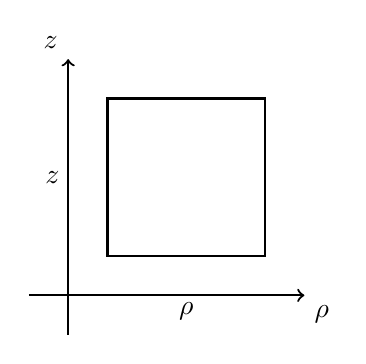
\begin{tikzpicture}
        % Eksenleri çiz
        \draw[thick, ->] (-0.5,0) -- (3,0) node[anchor=north west] {$\rho$};
        \draw[thick, ->] (0,-0.5) -- (0,3) node[anchor=south east] {$z$};

        % Dikdörtgen çiz
        \draw[thick] (0.5,0.5) rectangle (2.5,2.5);
        \node at (1.5, -0.2) {$ \rho $};
        \node at (-0.2, 1.5) {$ z $};
    \end{tikzpicture}
    \caption{$xz$ Düzleminde Dikdörtgen Levha}
    \label{fig:dikdortgen_levha}
\end{figure}

\textbf{2. Döndürme İşlemi:}

Bu levhayı $z$ ekseni etrafında $2\pi$ radyan (360 derece) döndürdüğümüzde, bir silindir elde ederiz. $\phi$ açısı, bu döndürme işlemini temsil eder.

\textbf{3. Silindirin Oluşumu:}

\begin{figure}[htbp]
    \centering
    \begin{tikzpicture}
        % Eksenleri çiz
        \draw[thick, ->] (-3,0) -- (3,0) node[anchor=north west] {x};
        \draw[thick, ->] (0,-3) -- (0,3) node[anchor=south east] {y};
        \draw[thick, ->] (0,0) -- (1.5,1.5) node[anchor=west] {z};

        % Silindir çiz
        \draw[dashed] (1,0) arc (0:360:1);
        \draw[dashed] (1,0) -- (1,2);
        \draw[dashed] (-1,0) -- (-1,2);
        \draw[dashed] (1,2) arc (0:360:1);
    \end{tikzpicture}
    \caption{Silindirik Koordinat Sistemi Oluşumu}
    \label{fig:silindir_olusumu}
\end{figure}

\textbf{4. Sınır Değerleri:}

Silindirik koordinatlarda, her bir değişkenin belirli sınır değerleri vardır:

\begin{itemize}
    \item $\rho$: Yarıçap her zaman pozitif veya sıfır olmalıdır: $\rho \geq 0$.
    \item $\phi$: Azimut açısı genellikle $0$ ile $2\pi$ arasında değişir: $0 \leq \phi < 2\pi$.
    \item $z$: Yükseklik, $-\infty$ ile $+\infty$ arasında herhangi bir değer alabilir: $-\infty < z < +\infty$.
\end{itemize}

\textbf{5. Farklı Döndürme Türleri ve Oluşan Şekiller:}

Eğer levhayı farklı şekillerde döndürürsek, farklı geometrik yapılar elde edebiliriz. Örneğin:

\begin{itemize}
    \item \textbf{Tam Döndürme ($2\pi$)}: $xz$ düzlemindeki dikdörtgenin $z$ ekseni etrafında tam olarak döndürülmesiyle elde edilen silindir.
    \item \textbf{Kısmi Döndürme ($\theta < 2\pi$)}: $xz$ düzlemindeki dikdörtgenin $z$ ekseni etrafında $\theta$ açısı kadar döndürülmesiyle elde edilen silindir parçası.
    \item \textbf{Öteleme}: $xz$ düzlemindeki dikdörtgenin $z$ ekseni boyunca ötelenmesiyle elde edilen prizma.
\end{itemize}

\begin{figure}[htbp]
    \centering
    \begin{tabular}{ccc}
         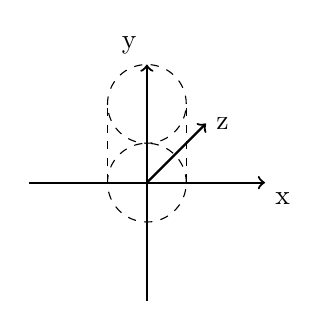
\begin{tikzpicture}[scale=0.5]
        % Eksenleri çiz
        \draw[thick, ->] (-3,0) -- (3,0) node[anchor=north west] {x};
        \draw[thick, ->] (0,-3) -- (0,3) node[anchor=south east] {y};
        \draw[thick, ->] (0,0) -- (1.5,1.5) node[anchor=west] {z};

        % Silindir çiz
        \draw[dashed] (1,0) arc (0:360:1);
        \draw[dashed] (1,0) -- (1,2);
        \draw[dashed] (-1,0) -- (-1,2);
        \draw[dashed] (1,2) arc (0:360:1);
    \end{tikzpicture}
    &
         \begin{tikzpicture}[scale=0.5]
        % Eksenleri çiz
        \draw[thick, ->] (-3,0) -- (3,0) node[anchor=north west] {x};
        \draw[thick, ->] (0,-3) -- (0,3) node[anchor=south east] {y};
        \draw[thick, ->] (0,0) -- (1.5,1.5) node[anchor=west] {z};

        % Silindir çiz
        \draw[dashed] (1,0) arc (0:180:1);
        \draw[dashed] (1,0) -- (1,2);
        \draw[dashed] (-1,0) -- (-1,2);
        \draw[dashed] (1,2) arc (0:180:1);
    \end{tikzpicture}
    &
         \begin{tikzpicture}[scale=0.5]
        % Eksenleri çiz
        \draw[thick, ->] (-3,0) -- (3,0) node[anchor=north west] {x};
        \draw[thick, ->] (0,-3) -- (0,3) node[anchor=south east] {y};
        \draw[thick, ->] (0,0) -- (1.5,1.5) node[anchor=west] {z};

        % Silindir çiz
        \draw[dashed] (1,0) -- (1,2);
        \draw[dashed] (-1,0) -- (-1,2);
        \draw[dashed] (-1,0) -- (1,0);
         \draw[dashed] (-1,2) -- (1,2);
    \end{tikzpicture}
    \\
    Tam Döndürme & Kısmi Döndürme & Öteleme
    \end{tabular}
    \caption{Farklı Döndürme Türleri}
    \label{fig:farkli_dondurme_turleri}
\end{figure}

Bu şemalar, silindirik koordinat sisteminin nasıl oluşturulduğunu ve farklı döndürme türlerinin hangi geometrik yapıları ortaya çıkardığını görsel olarak açıklamaktadır.

\end{document}
\documentclass[11pt,letterpaper,twocolumn]{fenbil}
\usepackage{amsmath}
\usepackage{amssymb}
\usepackage{graphicx}
\usepackage{tikz}
\title{FMM - Fizikte Matematiksel Metotlar - Ders Notları}
\author{Celal Ekrem Torun}
\date{6 Mart 2025}

\begin{document}
\twocolumn[\begin{@twocolumnfalse}

\begin{minipage}{0.15\textwidth}{
    }
\end{minipage}
\hspace{25pt}
\begin{minipage}{0.75\textwidth}
\vspace{5mm}
\Large{\textbf{FMM - Fizikte Matematiksel Metotlar - Ders 1 (6 Mart 2025)}}
    \vspace{3mm}
    
    \large{\textbf{Hazırlayan}; Celal Ekrem Torun}
    \vspace{2mm}
    
    \fontsize{0.35cm}{0.5cm}\selectfont \textit{Fizik Bölümü, İstanbul Üniversitesi\newline 
    Beyazıt, Fatih, İstanbul, Türkiye}
    
\end{minipage}

\small

\end{@twocolumnfalse}]

\section{Matematiksel Metotlar}

\textbf{Not:} 1 Mart'ta gradyen vektörü işlendi, 6 Mart'ta eğrisel koordinatlara başlanacak.

\subsection{Gradyen}

\textbf{Tanım:} Bir $\phi(x, y, z)$ skaler alanının gradyeni, o alanın en hızlı değişim yönünü ve büyüklüğünü gösteren bir vektör alanıdır.

Kartezyen koordinatlarda gradyen şu şekilde tanımlanır:

\[
\nabla \phi = \frac{\partial \phi}{\partial x} \hat{e_x} + \frac{\partial \phi}{\partial y} \hat{e_y} + \frac{\partial \phi}{\partial z} \hat{e_z}
\]

Burada:

\begin{itemize}
    \item $\nabla \phi$: Gradyen vektörü
    \item $\phi(x, y, z)$: Skaler alan
    \item $\hat{e_x}$, $\hat{e_y}$, $\hat{e_z}$: Sırasıyla $x$, $y$ ve $z$ yönlerindeki birim vektörler
\end{itemize}

\textbf{Önemli Not:} $\nabla \phi$, $\hat{e_x}$, $\hat{e_y}$ ve $\hat{e_z}$ ile ayrı ayrı skalar çarpılırsa, $\phi$ fonksiyonunun sınırları ile $x$, $y$ ve $z$ doğrultusundaki değişimi bulunur.

Bir $P(x,y,z)$ noktasındaki $\phi$ fonksiyonunun değişim oranı, $\nabla \phi \cdot d\vec{r}$ ile bulunur. Burada $d\vec{r}$, $P$ noktasından küçük bir yer değiştirmeyi temsil eden vektördür. Eğer $\phi = c_1$ yüzeyinden $\phi = c_2$ yüzeyine gidilirse, değişim $d\phi = c_2 - c_1$ olur ve $d\phi \neq 0$ olur.

Eğer $\nabla \phi \cdot d\vec{r} = d\phi = 0$ ise, $\nabla \phi$, $d\vec{r}$ vektörüne diktir. Bu durumda $\nabla \phi$, $\frac{\nabla \phi}{|\nabla \phi|}$ ile aynı yöndedir.

\subsection{Doğrultu Türevi}

\textbf{Tanım:} Bir $\phi(x,y,z)$ skaler alanının, bir $\vec{u}$ birim vektörü yönündeki doğrultu türevi, $\phi$'nin $\vec{u}$ yönündeki değişim oranını verir.

Doğrultu türevi şu şekilde tanımlanır:

\[
\frac{\partial \phi}{\partial u} = \nabla \phi \cdot \hat{u} = |\nabla \phi| |\hat{u}| \cos \theta
\]

Burada:
\begin{itemize}
    \item $\frac{\partial \phi}{\partial u}$: Doğrultu türevi
    \item $\nabla \phi$: Gradyen vektörü
    \item $\hat{u}$: Birim vektör
    \item $\theta$: $\nabla \phi$ ve $\hat{u}$ arasındaki açı
\end{itemize}

$\frac{\partial \phi}{\partial u}$, $\phi$'nin bir $P(x,y,z)$ noktasındaki $\vec{u}$ birim vektörü ile belirlenen doğrultudaki doğrultu türevidir.

$\frac{\partial \phi}{\partial u} = \nabla \phi \cdot \hat{u} = |\nabla \phi| \cos \theta$

\subsection{Örnek Soru}

$\phi(x, y, z) = x^2yz + 4z^2$ fonksiyonunun $P(1, -2, -1)$ noktasındaki $\vec{dr} = (2\hat{e_x} - \hat{e_y} - 2\hat{e_z})$ doğrultusundaki türevini bulun.

\textbf{Çözüm:}

\textit{Adım 1: Gradyeni hesaplayalım:}

$\nabla \phi = (2xyz) \hat{e_x} + (x^2z) \hat{e_y} + (x^2y + 8z) \hat{e_z}$

\textit{Adım 2: P(1, -2, -1) noktasındaki gradyeni hesaplayalım:}

$\nabla \phi |_P = (2(1)(-2)(-1)) \hat{e_x} + ((1)^2(-1)) \hat{e_y} + ((1)^2(-2) + 8(-1)) \hat{e_z} = 4 \hat{e_x} - \hat{e_y} - 10 \hat{e_z}$

\textit{Adım 3: $\vec{u}$ birim vektörünü bulalım:}

$|\vec{dr}| = \sqrt{2^2 + (-1)^2 + (-2)^2} = \sqrt{9} = 3$

$\hat{u} = \frac{\vec{dr}}{|\vec{dr}|} = \frac{2}{3} \hat{e_x} - \frac{1}{3} \hat{e_y} - \frac{2}{3} \hat{e_z}$

\textit{Adım 4: Doğrultu türevini hesaplayalım:}

$\frac{\partial \phi}{\partial u} = \nabla \phi \cdot \hat{u} = (4 \hat{e_x} - \hat{e_y} - 10 \hat{e_z}) \cdot (\frac{2}{3} \hat{e_x} - \frac{1}{3} \hat{e_y} - \frac{2}{3} \hat{e_z}) = \frac{8}{3} + \frac{1}{3} + \frac{20}{3} = \frac{29}{3} \approx 9.67$

\subsection{Eğrisel Koordinatlar}

Üç boyutlu Öklit uzayında, bir noktanın Kartezyen koordinatları $(x, y, z)$ ile ifade edilir. Şimdi, bu koordinatlara bağlı üç yeni değişken tanımlayalım:

\begin{equation}
u_1 = u_1(x, y, z)
\end{equation}
\begin{equation}
u_2 = u_2(x, y, z)
\end{equation}
\begin{equation}
u_3 = u_3(x, y, z)
\end{equation}

Bu yeni değişkenler, eğrisel koordinatları temsil eder.

\subsubsection{$u_1$, $u_2$, $u_3$'ün Bağımsız Fonksiyonlar Olması}

Lineer homojen bir sistemin sıfırdan farklı çözüme sahip olabilmesi için, katsayılar determinantının sıfıra eşit olması gerekmektedir. Şimdi, $u_1$, $u_2$, $u_3$'ün bağımsız fonksiyonlar olmasının ne anlama geldiğini inceleyelim.

$u_1(x, y, z)$, $u_2(x, y, z)$ ve $u_3(x, y, z)$ fonksiyonları için aşağıdaki ifadeler tanımlanır:

\begin{equation}
u_1 = u_1(x, y, z)
\end{equation}
\begin{equation}
u_2 = u_2(x, y, z)
\end{equation}
\begin{equation}
u_3 = u_3(x, y, z)
\end{equation}

Bu fonksiyonların diferansiyelleri ise şu şekildedir:

\begin{equation}
du_1 = \frac{\partial u_1}{\partial x} dx + \frac{\partial u_1}{\partial y} dy + \frac{\partial u_1}{\partial z} dz
\end{equation}
\begin{equation}
du_2 = \frac{\partial u_2}{\partial x} dx + \frac{\partial u_2}{\partial y} dy + \frac{\partial u_2}{\partial z} dz
\end{equation}
\begin{equation}
du_3 = \frac{\partial u_3}{\partial x} dx + \frac{\partial u_3}{\partial y} dy + \frac{\partial u_3}{\partial z} dz
\end{equation}

Bu denklemleri matris formunda ifade edebiliriz:

\begin{equation}
\begin{bmatrix} du_1 \\ du_2 \\ du_3 \end{bmatrix} = 
\begin{bmatrix}
\frac{\partial u_1}{\partial x} & \frac{\partial u_1}{\partial y} & \frac{\partial u_1}{\partial z} \\
\frac{\partial u_2}{\partial x} & \frac{\partial u_2}{\partial y} & \frac{\partial u_2}{\partial z} \\
\frac{\partial u_3}{\partial x} & \frac{\partial u_3}{\partial y} & \frac{\partial u_3}{\partial z}
\end{bmatrix}
\begin{bmatrix} dx \\ dy \\ dz \end{bmatrix}
\end{equation}

Bu matrisi daha kompakt bir şekilde ifade etmek için, aşağıdaki tanımlamaları yapalım:

\begin{equation}
d\mathbf{u} = \begin{bmatrix} du_1 \\ du_2 \\ du_3 \end{bmatrix}, \quad
A = \begin{bmatrix}
\frac{\partial u_1}{\partial x} & \frac{\partial u_1}{\partial y} & \frac{\partial u_1}{\partial z} \\
\frac{\partial u_2}{\partial x} & \frac{\partial u_2}{\partial y} & \frac{\partial u_2}{\partial z} \\
\frac{\partial u_3}{\partial x} & \frac{\partial u_3}{\partial y} & \frac{\partial u_3}{\partial z}
\end{bmatrix}, \quad
d\mathbf{x} = \begin{bmatrix} dx \\ dy \\ dz \end{bmatrix}
\end{equation}

Bu durumda, yukarıdaki denklem şu şekilde yazılabilir:

\begin{equation}
d\mathbf{u} = A \, d\mathbf{x}
\end{equation}

$dx$, $dy$ ve $dz$'yi $du_1$, $du_2$ ve $du_3$ cinsinden ifade etmek için, $A$ matrisinin tersini almamız gerekir:

\begin{equation}
d\mathbf{x} = A^{-1} \, d\mathbf{u}
\end{equation}

$A^{-1}$ matrisinin var olabilmesi için, $A$ matrisinin determinantı sıfırdan farklı olmalıdır:

\begin{equation}
J = \det(A) \neq 0
\end{equation}

Burada $J$, Jacobian determinantıdır. $A^{-1}$ matrisi, $A$'nın ek matrisinin determinantına bölünmesiyle bulunur:

\begin{equation}
A^{-1} = \frac{\text{adj}(A)}{J}
\end{equation}

Bu durumda, $dx$, $dy$ ve $dz$ aşağıdaki şekilde ifade edilebilir:

\begin{equation}
\begin{bmatrix} dx \\ dy \\ dz \end{bmatrix} = A^{-1} \begin{bmatrix} du_1 \\ du_2 \\ du_3 \end{bmatrix}
\end{equation}

Kartezyen koordinatları eğrisel koordinatlar cinsinden ifade etmek için, aşağıdaki bağıntıları kullanırız:

\begin{equation}
x = x(u_1, u_2, u_3)
\end{equation}
\begin{equation}
y = y(u_1, u_2, u_3)
\end{equation}
\begin{equation}
z = z(u_1, u_2, u_3)
\end{equation}

Bu durumda, konum vektörü $\vec{r}$ aşağıdaki gibi ifade edilir:

\begin{equation}
\vec{r} = x(u_1, u_2, u_3) \, \hat{e_x} + y(u_1, u_2, u_3) \, \hat{e_y} + z(u_1, u_2, u_3) \, \hat{e_z}
\end{equation}

\subsubsection{Eğrisel Koordinatların Geometrik Gösterimi}

Aşağıdaki şemalar, eğrisel koordinatların ve Kartezyen koordinat sisteminin ayrı ayrı gösterimlerini sunmaktadır.

\textbf{Kartezyen Koordinat Sistemi:}

\begin{figure}[htbp]
    \centering
    \begin{tikzpicture}
        \draw[thick, ->] (-3,0) -- (3,0) node[anchor=north west] {x};
        \draw[thick, ->] (0,-3) -- (0,3) node[anchor=south east] {y};
        \draw[thick, ->] (0,0) -- (1.5,1.5) node[anchor=west] {z};
        
        \node[below right] at (2.2, -0.2) {Apsis (x)};
        \node[above] at (-2.2, 0) {Ordinat (y)};
    \end{tikzpicture}
    \caption{Kartezyen Koordinat Sistemi}
    \label{fig:kartezyen_koordinat}
\end{figure}

Bu şemada:

\begin{itemize}
    \item \textit{Apsis (x)}: Yatay ekseni temsil eder.
    \item \textit{Ordinat (y)}: Dikey ekseni temsil eder.
    \item \textit{Kot (z)}: Derinlik eksenini temsil eder.
\end{itemize}

\textbf{Eğrisel Koordinat Sistemi Gösterimi:}

\begin{figure}[htbp]
    \centering
    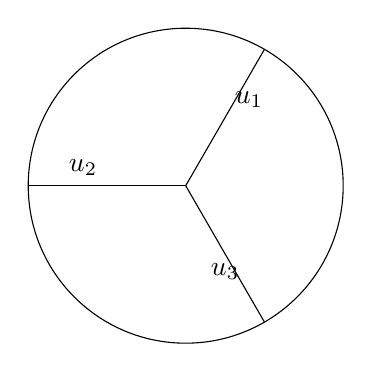
\begin{tikzpicture}
        \draw (0,0) circle (2cm);
        \draw (0,0) -- (60:2cm) node[midway, above right] {$u_1$};
        \draw (0,0) -- (180:2cm) node[midway, above left] {$u_2$};
        \draw (0,0) -- (300:2cm) node[midway, below] {$u_3$};
    \end{tikzpicture}
    \caption{Eğrisel Koordinat Sistemi}
    \label{fig:egrisel_koordinat}
\end{figure}

Bu şema, eğrisel koordinatları $(u_1, u_2, u_3)$ temsil eden bir dairesel gösterim sunar. Bu gösterim, eğrisel koordinatların Kartezyen koordinat sistemi ile ilişkisini anlamak için kullanılabilir.

Eğrisel koordinatlar, belirli bir probleme daha uygun bir koordinat sistemi seçme esnekliği sağlar. Örneğin, silindirik veya küresel koordinatlar, belirli simetrilere sahip problemleri çözmek için daha uygun olabilir.

\subsection{Eğrisel Koordinat Örnekleri}

\subsubsection{Silindirik Koordinatlar $(\rho, \phi, z)$}

Silindirik koordinatlar, üç boyutlu uzayı tanımlamak için kullanılan bir koordinat sistemidir. Bu sistemde, bir noktanın konumu, bir eksene olan uzaklığı $(\rho)$, bu eksen etrafındaki açısı $(\phi)$ ve eksen üzerindeki yüksekliği $(z)$ ile belirlenir.

\textbf{Tanımlar:}

\begin{itemize}
    \item \textit{$\rho$ (rho)}: $xy$ düzlemindeki orijinden olan uzaklık.
    \item \textit{$\phi$ (phi)}: $x$ ekseni ile $\rho$ arasındaki açı (azimut açısı).
    \item \textit{$z$}: $z$ ekseni üzerindeki yükseklik.
\end{itemize}

\textbf{Kartezyen ve Silindirik Koordinatlar Arasındaki İlişki:}

Kartezyen koordinatlardaki $(x, y, z)$ noktası ile silindirik koordinatlardaki $(\rho, \phi, z)$ noktası arasındaki dönüşüm aşağıdaki gibidir:

\begin{itemize}
    \item $x = \rho \cos \phi$
    \item $y = \rho \sin \phi$
    \item $z = z$
\end{itemize}

\textbf{Dönüşümün Tersi:}

\begin{itemize}
    \item $\rho = \sqrt{x^2 + y^2}$
    \item $\phi = \arctan \left( \frac{y}{x} \right)$
    \item $z = z$
\end{itemize}

\textbf{Geometrik Gösterim:}

\begin{figure}[htbp]
    \centering
    \begin{tikzpicture}
        % Eksenleri çiz
        \draw[thick, ->] (-3,0) -- (3,0) node[anchor=north west] {x};
        \draw[thick, ->] (0,-3) -- (0,3) node[anchor=south east] {y};
        \draw[thick, ->] (0,0) -- (1.5,1.5) node[anchor=west] {z};

        % Silindir çiz
        \draw[dashed] (1,0) arc (0:360:1);
        \draw[dashed] (1,0) -- (1,2);
        \draw[dashed] (-1,0) -- (-1,2);
        \draw[dashed] (1,2) arc (0:360:1);

        % P noktası
        \node[circle, fill, inner sep=1.5pt, label=above right:$P$] (P) at (0.7, 1, 1) {};

        % P' noktası
        \node[circle, fill, inner sep=1.5pt, label=below:$P'$] (Pp) at (0.7,0,0) {};

        % rho
        \draw[dashed] (0,0) -- (Pp) node[midway, below] {$\rho$};

        % z
        \draw[dashed] (Pp) -- (P) node[midway, right] {$z$};

        % Açı phi
        \draw (0.4,0) arc (0:45:0.4);
        \node at (0.7,0.3) {$\phi$};

    \end{tikzpicture}
    \caption{Silindirik Koordinat Sistemi}
    \label{fig:silindirik_koordinat}
\end{figure}

Bu şemada:

\begin{itemize}
    \item $P$: Uzaydaki bir noktayı temsil eder.
    \item $P'$: $P$ noktasının $xy$ düzlemindeki izdüşümüdür.
    \item $\rho$: $P'$ noktasının orijine olan uzaklığıdır.
    \item $\phi$: $x$ ekseni ile $OP'$ arasındaki açıdır (azimut açısı).
    \item $z$: $P$ noktasının $z$ ekseni üzerindeki yüksekliğidir.
\end{itemize}

\textbf{Jacobian Dönüşümü:}

Silindirik koordinatlardaki $(\rho, \phi, z)$ ile Kartezyen koordinatlardaki $(x, y, z)$ arasındaki ilişki aşağıdaki gibidir:

\begin{itemize}
    \item $x = \rho \cos \phi$
    \item $y = \rho \sin \phi$
    \item $z = z$
\end{itemize}

Burada $\phi$, azimut açısını temsil etmektedir.

Bu dönüşümü ifade etmek için Jacobian matrisini kullanabiliriz. Jacobian matrisi, koordinat dönüşümünün kısmi türevlerini içerir:

\begin{equation}
J = \begin{bmatrix}
\frac{\partial x}{\partial \rho} & \frac{\partial x}{\partial \phi} & \frac{\partial x}{\partial z} \\
\frac{\partial y}{\partial \rho} & \frac{\partial y}{\partial \phi} & \frac{\partial y}{\partial z} \\
\frac{\partial z}{\partial \rho} & \frac{\partial z}{\partial \phi} & \frac{\partial z}{\partial z}
\end{bmatrix}
\end{equation}

Bu matrisin elemanlarını hesaplarsak:

\begin{itemize}
    \item $\frac{\partial x}{\partial \rho} = \cos \phi$
    \item $\frac{\partial x}{\partial \phi} = -\rho \sin \phi$
    \item $\frac{\partial x}{\partial z} = 0$
    \item $\frac{\partial y}{\partial \rho} = \sin \phi$
    \item $\frac{\partial y}{\partial \phi} = \rho \cos \phi$
    \item $\frac{\partial y}{\partial z} = 0$
    \item $\frac{\partial z}{\partial \rho} = 0$
    \item $\frac{\partial z}{\partial \phi} = 0$
    \item $\frac{\partial z}{\partial z} = 1$
\end{itemize}

Bu değerleri Jacobian matrisine yerleştirdiğimizde:

\begin{equation}
J = \begin{bmatrix}
\cos \phi & -\rho \sin \phi & 0 \\
\sin \phi & \rho \cos \phi & 0 \\
0 & 0 & 1
\end{bmatrix}
\end{equation}

Jacobian determinantı ise şu şekilde hesaplanır:

\begin{equation}
\det(J) = \rho \cos^2 \phi + \rho \sin^2 \phi = \rho (\cos^2 \phi + \sin^2 \phi) = \rho
\end{equation}

Burada $\rho = \sqrt{x^2 + y^2}$ ve $\rho \neq 0$ olmalıdır.

Ayrıca, $\phi = \arctan \left( \frac{y}{x} \right)$ ifadesi kullanılır.

$z = z$ olduğundan, $z$ için türev dönüşümleri basittir.

Bu Jacobian determinantı, hacim elemanının dönüşümünde kullanılır:

\begin{equation}
dV = dx \, dy \, dz = |J| \, d\rho \, d\phi \, dz = \rho \, d\rho \, d\phi \, dz
\end{equation}

Bu dönüşümler, koordinatları bir sistemden diğerine dönüştürmek için kullanılır. Jacobian determinantı, dönüşümün hacim elemanını nasıl etkilediğini gösterir.

\textbf{Silindirik Koordinatların Oluşumu ve Sınır Değerleri}

Silindirik koordinat sistemi, bir levhanın (dikdörtgenin) bir eksen etrafında döndürülmesiyle görselleştirilebilir. Bu bölümde, bu dönüşümün nasıl gerçekleştiğini ve silindirik koordinatların sınır değerlerini inceleyeceğiz.

\textbf{1. Levhanın (Dikdörtgenin) Çizimi:}

İlk olarak, $xz$ düzleminde bir levha (dikdörtgen) çizelim. Bu levha, silindirin yüksekliğini $(z)$ ve yarıçapını $(\rho)$ temsil edecektir.

\begin{figure}[htbp]
    \centering
    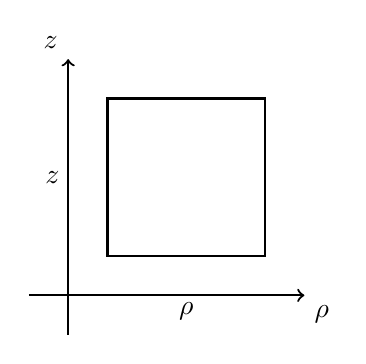
\begin{tikzpicture}
        % Eksenleri çiz
        \draw[thick, ->] (-0.5,0) -- (3,0) node[anchor=north west] {$\rho$};
        \draw[thick, ->] (0,-0.5) -- (0,3) node[anchor=south east] {$z$};

        % Dikdörtgen çiz
        \draw[thick] (0.5,0.5) rectangle (2.5,2.5);
        \node at (1.5, -0.2) {$ \rho $};
        \node at (-0.2, 1.5) {$ z $};
    \end{tikzpicture}
    \caption{$xz$ Düzleminde Dikdörtgen Levha}
    \label{fig:dikdortgen_levha}
\end{figure}

\textbf{2. Döndürme İşlemi:}

Bu levhayı $z$ ekseni etrafında $2\pi$ radyan (360 derece) döndürdüğümüzde, bir silindir elde ederiz. $\phi$ açısı, bu döndürme işlemini temsil eder.

\textbf{3. Silindirin Oluşumu:}

\begin{figure}[htbp]
    \centering
    \begin{tikzpicture}
        % Eksenleri çiz
        \draw[thick, ->] (-3,0) -- (3,0) node[anchor=north west] {x};
        \draw[thick, ->] (0,-3) -- (0,3) node[anchor=south east] {y};
        \draw[thick, ->] (0,0) -- (1.5,1.5) node[anchor=west] {z};

        % Silindir çiz
        \draw[dashed] (1,0) arc (0:360:1);
        \draw[dashed] (1,0) -- (1,2);
        \draw[dashed] (-1,0) -- (-1,2);
        \draw[dashed] (1,2) arc (0:360:1);
    \end{tikzpicture}
    \caption{Silindirik Koordinat Sistemi Oluşumu}
    \label{fig:silindir_olusumu}
\end{figure}

\textbf{4. Sınır Değerleri:}

Silindirik koordinatlarda, her bir değişkenin belirli sınır değerleri vardır:

\begin{itemize}
    \item $\rho$: Yarıçap her zaman pozitif veya sıfır olmalıdır: $\rho \geq 0$.
    \item $\phi$: Azimut açısı genellikle $0$ ile $2\pi$ arasında değişir: $0 \leq \phi < 2\pi$.
    \item $z$: Yükseklik, $-\infty$ ile $+\infty$ arasında herhangi bir değer alabilir: $-\infty < z < +\infty$.
\end{itemize}

\textbf{5. Farklı Döndürme Türleri ve Oluşan Şekiller:}

Eğer levhayı farklı şekillerde döndürürsek, farklı geometrik yapılar elde edebiliriz. Örneğin:

\begin{itemize}
    \item \textbf{Tam Döndürme ($2\pi$)}: $xz$ düzlemindeki dikdörtgenin $z$ ekseni etrafında tam olarak döndürülmesiyle elde edilen silindir.
    \item \textbf{Kısmi Döndürme ($\theta < 2\pi$)}: $xz$ düzlemindeki dikdörtgenin $z$ ekseni etrafında $\theta$ açısı kadar döndürülmesiyle elde edilen silindir parçası.
    \item \textbf{Öteleme}: $xz$ düzlemindeki dikdörtgenin $z$ ekseni boyunca ötelenmesiyle elde edilen prizma.
\end{itemize}

\begin{figure}[htbp]
    \centering
    \begin{tabular}{ccc}
         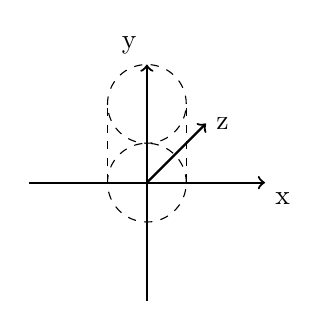
\begin{tikzpicture}[scale=0.5]
        % Eksenleri çiz
        \draw[thick, ->] (-3,0) -- (3,0) node[anchor=north west] {x};
        \draw[thick, ->] (0,-3) -- (0,3) node[anchor=south east] {y};
        \draw[thick, ->] (0,0) -- (1.5,1.5) node[anchor=west] {z};

        % Silindir çiz
        \draw[dashed] (1,0) arc (0:360:1);
        \draw[dashed] (1,0) -- (1,2);
        \draw[dashed] (-1,0) -- (-1,2);
        \draw[dashed] (1,2) arc (0:360:1);
    \end{tikzpicture}
    &
         \begin{tikzpicture}[scale=0.5]
        % Eksenleri çiz
        \draw[thick, ->] (-3,0) -- (3,0) node[anchor=north west] {x};
        \draw[thick, ->] (0,-3) -- (0,3) node[anchor=south east] {y};
        \draw[thick, ->] (0,0) -- (1.5,1.5) node[anchor=west] {z};

        % Silindir çiz
        \draw[dashed] (1,0) arc (0:180:1);
        \draw[dashed] (1,0) -- (1,2);
        \draw[dashed] (-1,0) -- (-1,2);
        \draw[dashed] (1,2) arc (0:180:1);
    \end{tikzpicture}
    &
         \begin{tikzpicture}[scale=0.5]
        % Eksenleri çiz
        \draw[thick, ->] (-3,0) -- (3,0) node[anchor=north west] {x};
        \draw[thick, ->] (0,-3) -- (0,3) node[anchor=south east] {y};
        \draw[thick, ->] (0,0) -- (1.5,1.5) node[anchor=west] {z};

        % Silindir çiz
        \draw[dashed] (1,0) -- (1,2);
        \draw[dashed] (-1,0) -- (-1,2);
        \draw[dashed] (-1,0) -- (1,0);
         \draw[dashed] (-1,2) -- (1,2);
    \end{tikzpicture}
    \\
    Tam Döndürme & Kısmi Döndürme & Öteleme
    \end{tabular}
    \caption{Farklı Döndürme Türleri}
    \label{fig:farkli_dondurme_turleri}
\end{figure}

Bu şemalar, silindirik koordinat sisteminin nasıl oluşturulduğunu ve farklı döndürme türlerinin hangi geometrik yapıları ortaya çıkardığını görsel olarak açıklamaktadır.

\end{document}
\documentclass[11pt,letterpaper,twocolumn]{fenbil}
\usepackage{amsmath}
\usepackage{amssymb}
\usepackage{graphicx}
\usepackage{tikz}
\title{FMM - Fizikte Matematiksel Metotlar - Ders Notları}
\author{Celal Ekrem Torun}
\date{6 Mart 2025}

\begin{document}
\twocolumn[\begin{@twocolumnfalse}

\begin{minipage}{0.15\textwidth}{
    }
\end{minipage}
\hspace{25pt}
\begin{minipage}{0.75\textwidth}
\vspace{5mm}
\Large{\textbf{FMM - Fizikte Matematiksel Metotlar - Ders 1 (6 Mart 2025)}}
    \vspace{3mm}
    
    \large{\textbf{Hazırlayan}; Celal Ekrem Torun}
    \vspace{2mm}
    
    \fontsize{0.35cm}{0.5cm}\selectfont \textit{Fizik Bölümü, İstanbul Üniversitesi\newline 
    Beyazıt, Fatih, İstanbul, Türkiye}
    
\end{minipage}

\small

\end{@twocolumnfalse}]

\section{Matematiksel Metotlar}

\textbf{Not:} 1 Mart'ta gradyen vektörü işlendi, 6 Mart'ta eğrisel koordinatlara başlanacak.

\subsection{Gradyen}

\textbf{Tanım:} Bir $\phi(x, y, z)$ skaler alanının gradyeni, o alanın en hızlı değişim yönünü ve büyüklüğünü gösteren bir vektör alanıdır.

Kartezyen koordinatlarda gradyen şu şekilde tanımlanır:

\[
\nabla \phi = \frac{\partial \phi}{\partial x} \hat{e_x} + \frac{\partial \phi}{\partial y} \hat{e_y} + \frac{\partial \phi}{\partial z} \hat{e_z}
\]

Burada:

\begin{itemize}
    \item $\nabla \phi$: Gradyen vektörü
    \item $\phi(x, y, z)$: Skaler alan
    \item $\hat{e_x}$, $\hat{e_y}$, $\hat{e_z}$: Sırasıyla $x$, $y$ ve $z$ yönlerindeki birim vektörler
\end{itemize}

\textbf{Önemli Not:} $\nabla \phi$, $\hat{e_x}$, $\hat{e_y}$ ve $\hat{e_z}$ ile ayrı ayrı skalar çarpılırsa, $\phi$ fonksiyonunun sınırları ile $x$, $y$ ve $z$ doğrultusundaki değişimi bulunur.

Bir $P(x,y,z)$ noktasındaki $\phi$ fonksiyonunun değişim oranı, $\nabla \phi \cdot d\vec{r}$ ile bulunur. Burada $d\vec{r}$, $P$ noktasından küçük bir yer değiştirmeyi temsil eden vektördür. Eğer $\phi = c_1$ yüzeyinden $\phi = c_2$ yüzeyine gidilirse, değişim $d\phi = c_2 - c_1$ olur ve $d\phi \neq 0$ olur.

Eğer $\nabla \phi \cdot d\vec{r} = d\phi = 0$ ise, $\nabla \phi$, $d\vec{r}$ vektörüne diktir. Bu durumda $\nabla \phi$, $\frac{\nabla \phi}{|\nabla \phi|}$ ile aynı yöndedir.

\subsection{Doğrultu Türevi}

\textbf{Tanım:} Bir $\phi(x,y,z)$ skaler alanının, bir $\vec{u}$ birim vektörü yönündeki doğrultu türevi, $\phi$'nin $\vec{u}$ yönündeki değişim oranını verir.

Doğrultu türevi şu şekilde tanımlanır:

\[
\frac{\partial \phi}{\partial u} = \nabla \phi \cdot \hat{u} = |\nabla \phi| |\hat{u}| \cos \theta
\]

Burada:
\begin{itemize}
    \item $\frac{\partial \phi}{\partial u}$: Doğrultu türevi
    \item $\nabla \phi$: Gradyen vektörü
    \item $\hat{u}$: Birim vektör
    \item $\theta$: $\nabla \phi$ ve $\hat{u}$ arasındaki açı
\end{itemize}

$\frac{\partial \phi}{\partial u}$, $\phi$'nin bir $P(x,y,z)$ noktasındaki $\vec{u}$ birim vektörü ile belirlenen doğrultudaki doğrultu türevidir.

$\frac{\partial \phi}{\partial u} = \nabla \phi \cdot \hat{u} = |\nabla \phi| \cos \theta$

\subsection{Örnek Soru}

$\phi(x, y, z) = x^2yz + 4z^2$ fonksiyonunun $P(1, -2, -1)$ noktasındaki $\vec{dr} = (2\hat{e_x} - \hat{e_y} - 2\hat{e_z})$ doğrultusundaki türevini bulun.

\textbf{Çözüm:}

\textit{Adım 1: Gradyeni hesaplayalım:}

$\nabla \phi = (2xyz) \hat{e_x} + (x^2z) \hat{e_y} + (x^2y + 8z) \hat{e_z}$

\textit{Adım 2: P(1, -2, -1) noktasındaki gradyeni hesaplayalım:}

$\nabla \phi |_P = (2(1)(-2)(-1)) \hat{e_x} + ((1)^2(-1)) \hat{e_y} + ((1)^2(-2) + 8(-1)) \hat{e_z} = 4 \hat{e_x} - \hat{e_y} - 10 \hat{e_z}$

\textit{Adım 3: $\vec{u}$ birim vektörünü bulalım:}

$|\vec{dr}| = \sqrt{2^2 + (-1)^2 + (-2)^2} = \sqrt{9} = 3$

$\hat{u} = \frac{\vec{dr}}{|\vec{dr}|} = \frac{2}{3} \hat{e_x} - \frac{1}{3} \hat{e_y} - \frac{2}{3} \hat{e_z}$

\textit{Adım 4: Doğrultu türevini hesaplayalım:}

$\frac{\partial \phi}{\partial u} = \nabla \phi \cdot \hat{u} = (4 \hat{e_x} - \hat{e_y} - 10 \hat{e_z}) \cdot (\frac{2}{3} \hat{e_x} - \frac{1}{3} \hat{e_y} - \frac{2}{3} \hat{e_z}) = \frac{8}{3} + \frac{1}{3} + \frac{20}{3} = \frac{29}{3} \approx 9.67$

\subsection{Eğrisel Koordinatlar}

Üç boyutlu Öklit uzayında, bir noktanın Kartezyen koordinatları $(x, y, z)$ ile ifade edilir. Şimdi, bu koordinatlara bağlı üç yeni değişken tanımlayalım:

\begin{equation}
u_1 = u_1(x, y, z)
\end{equation}
\begin{equation}
u_2 = u_2(x, y, z)
\end{equation}
\begin{equation}
u_3 = u_3(x, y, z)
\end{equation}

Bu yeni değişkenler, eğrisel koordinatları temsil eder.

\subsubsection{$u_1$, $u_2$, $u_3$'ün Bağımsız Fonksiyonlar Olması}

Lineer homojen bir sistemin sıfırdan farklı çözüme sahip olabilmesi için, katsayılar determinantının sıfıra eşit olması gerekmektedir. Şimdi, $u_1$, $u_2$, $u_3$'ün bağımsız fonksiyonlar olmasının ne anlama geldiğini inceleyelim.

$u_1(x, y, z)$, $u_2(x, y, z)$ ve $u_3(x, y, z)$ fonksiyonları için aşağıdaki ifadeler tanımlanır:

\begin{equation}
u_1 = u_1(x, y, z)
\end{equation}
\begin{equation}
u_2 = u_2(x, y, z)
\end{equation}
\begin{equation}
u_3 = u_3(x, y, z)
\end{equation}

Bu fonksiyonların diferansiyelleri ise şu şekildedir:

\begin{equation}
du_1 = \frac{\partial u_1}{\partial x} dx + \frac{\partial u_1}{\partial y} dy + \frac{\partial u_1}{\partial z} dz
\end{equation}
\begin{equation}
du_2 = \frac{\partial u_2}{\partial x} dx + \frac{\partial u_2}{\partial y} dy + \frac{\partial u_2}{\partial z} dz
\end{equation}
\begin{equation}
du_3 = \frac{\partial u_3}{\partial x} dx + \frac{\partial u_3}{\partial y} dy + \frac{\partial u_3}{\partial z} dz
\end{equation}

Bu denklemleri matris formunda ifade edebiliriz:

\begin{equation}
\begin{bmatrix} du_1 \\ du_2 \\ du_3 \end{bmatrix} = 
\begin{bmatrix}
\frac{\partial u_1}{\partial x} & \frac{\partial u_1}{\partial y} & \frac{\partial u_1}{\partial z} \\
\frac{\partial u_2}{\partial x} & \frac{\partial u_2}{\partial y} & \frac{\partial u_2}{\partial z} \\
\frac{\partial u_3}{\partial x} & \frac{\partial u_3}{\partial y} & \frac{\partial u_3}{\partial z}
\end{bmatrix}
\begin{bmatrix} dx \\ dy \\ dz \end{bmatrix}
\end{equation}

Bu matrisi daha kompakt bir şekilde ifade etmek için, aşağıdaki tanımlamaları yapalım:

\begin{equation}
d\mathbf{u} = \begin{bmatrix} du_1 \\ du_2 \\ du_3 \end{bmatrix}, \quad
A = \begin{bmatrix}
\frac{\partial u_1}{\partial x} & \frac{\partial u_1}{\partial y} & \frac{\partial u_1}{\partial z} \\
\frac{\partial u_2}{\partial x} & \frac{\partial u_2}{\partial y} & \frac{\partial u_2}{\partial z} \\
\frac{\partial u_3}{\partial x} & \frac{\partial u_3}{\partial y} & \frac{\partial u_3}{\partial z}
\end{bmatrix}, \quad
d\mathbf{x} = \begin{bmatrix} dx \\ dy \\ dz \end{bmatrix}
\end{equation}

Bu durumda, yukarıdaki denklem şu şekilde yazılabilir:

\begin{equation}
d\mathbf{u} = A \, d\mathbf{x}
\end{equation}

$dx$, $dy$ ve $dz$'yi $du_1$, $du_2$ ve $du_3$ cinsinden ifade etmek için, $A$ matrisinin tersini almamız gerekir:

\begin{equation}
d\mathbf{x} = A^{-1} \, d\mathbf{u}
\end{equation}

$A^{-1}$ matrisinin var olabilmesi için, $A$ matrisinin determinantı sıfırdan farklı olmalıdır:

\begin{equation}
J = \det(A) \neq 0
\end{equation}

Burada $J$, Jacobian determinantıdır. $A^{-1}$ matrisi, $A$'nın ek matrisinin determinantına bölünmesiyle bulunur:

\begin{equation}
A^{-1} = \frac{\text{adj}(A)}{J}
\end{equation}

Bu durumda, $dx$, $dy$ ve $dz$ aşağıdaki şekilde ifade edilebilir:

\begin{equation}
\begin{bmatrix} dx \\ dy \\ dz \end{bmatrix} = A^{-1} \begin{bmatrix} du_1 \\ du_2 \\ du_3 \end{bmatrix}
\end{equation}

Kartezyen koordinatları eğrisel koordinatlar cinsinden ifade etmek için, aşağıdaki bağıntıları kullanırız:

\begin{equation}
x = x(u_1, u_2, u_3)
\end{equation}
\begin{equation}
y = y(u_1, u_2, u_3)
\end{equation}
\begin{equation}
z = z(u_1, u_2, u_3)
\end{equation}

Bu durumda, konum vektörü $\vec{r}$ aşağıdaki gibi ifade edilir:

\begin{equation}
\vec{r} = x(u_1, u_2, u_3) \, \hat{e_x} + y(u_1, u_2, u_3) \, \hat{e_y} + z(u_1, u_2, u_3) \, \hat{e_z}
\end{equation}

\subsubsection{Eğrisel Koordinatların Geometrik Gösterimi}

Aşağıdaki şemalar, eğrisel koordinatların ve Kartezyen koordinat sisteminin ayrı ayrı gösterimlerini sunmaktadır.

\textbf{Kartezyen Koordinat Sistemi:}

\begin{figure}[htbp]
    \centering
    \begin{tikzpicture}
        \draw[thick, ->] (-3,0) -- (3,0) node[anchor=north west] {x};
        \draw[thick, ->] (0,-3) -- (0,3) node[anchor=south east] {y};
        \draw[thick, ->] (0,0) -- (1.5,1.5) node[anchor=west] {z};
        
        \node[below right] at (2.2, -0.2) {Apsis (x)};
        \node[above] at (-2.2, 0) {Ordinat (y)};
    \end{tikzpicture}
    \caption{Kartezyen Koordinat Sistemi}
    \label{fig:kartezyen_koordinat}
\end{figure}

Bu şemada:

\begin{itemize}
    \item \textit{Apsis (x)}: Yatay ekseni temsil eder.
    \item \textit{Ordinat (y)}: Dikey ekseni temsil eder.
    \item \textit{Kot (z)}: Derinlik eksenini temsil eder.
\end{itemize}

\textbf{Eğrisel Koordinat Sistemi Gösterimi:}

\begin{figure}[htbp]
    \centering
    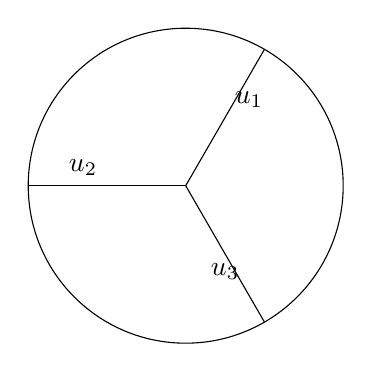
\begin{tikzpicture}
        \draw (0,0) circle (2cm);
        \draw (0,0) -- (60:2cm) node[midway, above right] {$u_1$};
        \draw (0,0) -- (180:2cm) node[midway, above left] {$u_2$};
        \draw (0,0) -- (300:2cm) node[midway, below] {$u_3$};
    \end{tikzpicture}
    \caption{Eğrisel Koordinat Sistemi}
    \label{fig:egrisel_koordinat}
\end{figure}

Bu şema, eğrisel koordinatları $(u_1, u_2, u_3)$ temsil eden bir dairesel gösterim sunar. Bu gösterim, eğrisel koordinatların Kartezyen koordinat sistemi ile ilişkisini anlamak için kullanılabilir.

Eğrisel koordinatlar, belirli bir probleme daha uygun bir koordinat sistemi seçme esnekliği sağlar. Örneğin, silindirik veya küresel koordinatlar, belirli simetrilere sahip problemleri çözmek için daha uygun olabilir.

\subsection{Eğrisel Koordinat Örnekleri}

\subsubsection{Silindirik Koordinatlar $(\rho, \phi, z)$}

Silindirik koordinatlar, üç boyutlu uzayı tanımlamak için kullanılan bir koordinat sistemidir. Bu sistemde, bir noktanın konumu, bir eksene olan uzaklığı $(\rho)$, bu eksen etrafındaki açısı $(\phi)$ ve eksen üzerindeki yüksekliği $(z)$ ile belirlenir.

\textbf{Tanımlar:}

\begin{itemize}
    \item \textit{$\rho$ (rho)}: $xy$ düzlemindeki orijinden olan uzaklık.
    \item \textit{$\phi$ (phi)}: $x$ ekseni ile $\rho$ arasındaki açı (azimut açısı).
    \item \textit{$z$}: $z$ ekseni üzerindeki yükseklik.
\end{itemize}

\textbf{Kartezyen ve Silindirik Koordinatlar Arasındaki İlişki:}

Kartezyen koordinatlardaki $(x, y, z)$ noktası ile silindirik koordinatlardaki $(\rho, \phi, z)$ noktası arasındaki dönüşüm aşağıdaki gibidir:

\begin{itemize}
    \item $x = \rho \cos \phi$
    \item $y = \rho \sin \phi$
    \item $z = z$
\end{itemize}

\textbf{Dönüşümün Tersi:}

\begin{itemize}
    \item $\rho = \sqrt{x^2 + y^2}$
    \item $\phi = \arctan \left( \frac{y}{x} \right)$
    \item $z = z$
\end{itemize}

\textbf{Geometrik Gösterim:}

\begin{figure}[htbp]
    \centering
    \begin{tikzpicture}
        % Eksenleri çiz
        \draw[thick, ->] (-3,0) -- (3,0) node[anchor=north west] {x};
        \draw[thick, ->] (0,-3) -- (0,3) node[anchor=south east] {y};
        \draw[thick, ->] (0,0) -- (1.5,1.5) node[anchor=west] {z};

        % Silindir çiz
        \draw[dashed] (1,0) arc (0:360:1);
        \draw[dashed] (1,0) -- (1,2);
        \draw[dashed] (-1,0) -- (-1,2);
        \draw[dashed] (1,2) arc (0:360:1);

        % P noktası
        \node[circle, fill, inner sep=1.5pt, label=above right:$P$] (P) at (0.7, 1, 1) {};

        % P' noktası
        \node[circle, fill, inner sep=1.5pt, label=below:$P'$] (Pp) at (0.7,0,0) {};

        % rho
        \draw[dashed] (0,0) -- (Pp) node[midway, below] {$\rho$};

        % z
        \draw[dashed] (Pp) -- (P) node[midway, right] {$z$};

        % Açı phi
        \draw (0.4,0) arc (0:45:0.4);
        \node at (0.7,0.3) {$\phi$};

    \end{tikzpicture}
    \caption{Silindirik Koordinat Sistemi}
    \label{fig:silindirik_koordinat}
\end{figure}

Bu şemada:

\begin{itemize}
    \item $P$: Uzaydaki bir noktayı temsil eder.
    \item $P'$: $P$ noktasının $xy$ düzlemindeki izdüşümüdür.
    \item $\rho$: $P'$ noktasının orijine olan uzaklığıdır.
    \item $\phi$: $x$ ekseni ile $OP'$ arasındaki açıdır (azimut açısı).
    \item $z$: $P$ noktasının $z$ ekseni üzerindeki yüksekliğidir.
\end{itemize}

\textbf{Jacobian Dönüşümü:}

Silindirik koordinatlardaki $(\rho, \phi, z)$ ile Kartezyen koordinatlardaki $(x, y, z)$ arasındaki ilişki aşağıdaki gibidir:

\begin{itemize}
    \item $x = \rho \cos \phi$
    \item $y = \rho \sin \phi$
    \item $z = z$
\end{itemize}

Burada $\phi$, azimut açısını temsil etmektedir.

Bu dönüşümü ifade etmek için Jacobian matrisini kullanabiliriz. Jacobian matrisi, koordinat dönüşümünün kısmi türevlerini içerir:

\begin{equation}
J = \begin{bmatrix}
\frac{\partial x}{\partial \rho} & \frac{\partial x}{\partial \phi} & \frac{\partial x}{\partial z} \\
\frac{\partial y}{\partial \rho} & \frac{\partial y}{\partial \phi} & \frac{\partial y}{\partial z} \\
\frac{\partial z}{\partial \rho} & \frac{\partial z}{\partial \phi} & \frac{\partial z}{\partial z}
\end{bmatrix}
\end{equation}

Bu matrisin elemanlarını hesaplarsak:

\begin{itemize}
    \item $\frac{\partial x}{\partial \rho} = \cos \phi$
    \item $\frac{\partial x}{\partial \phi} = -\rho \sin \phi$
    \item $\frac{\partial x}{\partial z} = 0$
    \item $\frac{\partial y}{\partial \rho} = \sin \phi$
    \item $\frac{\partial y}{\partial \phi} = \rho \cos \phi$
    \item $\frac{\partial y}{\partial z} = 0$
    \item $\frac{\partial z}{\partial \rho} = 0$
    \item $\frac{\partial z}{\partial \phi} = 0$
    \item $\frac{\partial z}{\partial z} = 1$
\end{itemize}

Bu değerleri Jacobian matrisine yerleştirdiğimizde:

\begin{equation}
J = \begin{bmatrix}
\cos \phi & -\rho \sin \phi & 0 \\
\sin \phi & \rho \cos \phi & 0 \\
0 & 0 & 1
\end{bmatrix}
\end{equation}

Jacobian determinantı ise şu şekilde hesaplanır:

\begin{equation}
\det(J) = \rho \cos^2 \phi + \rho \sin^2 \phi = \rho (\cos^2 \phi + \sin^2 \phi) = \rho
\end{equation}

Burada $\rho = \sqrt{x^2 + y^2}$ ve $\rho \neq 0$ olmalıdır.

Ayrıca, $\phi = \arctan \left( \frac{y}{x} \right)$ ifadesi kullanılır.

$z = z$ olduğundan, $z$ için türev dönüşümleri basittir.

Bu Jacobian determinantı, hacim elemanının dönüşümünde kullanılır:

\begin{equation}
dV = dx \, dy \, dz = |J| \, d\rho \, d\phi \, dz = \rho \, d\rho \, d\phi \, dz
\end{equation}

Bu dönüşümler, koordinatları bir sistemden diğerine dönüştürmek için kullanılır. Jacobian determinantı, dönüşümün hacim elemanını nasıl etkilediğini gösterir.

\textbf{Silindirik Koordinatların Oluşumu ve Sınır Değerleri}

Silindirik koordinat sistemi, bir levhanın (dikdörtgenin) bir eksen etrafında döndürülmesiyle görselleştirilebilir. Bu bölümde, bu dönüşümün nasıl gerçekleştiğini ve silindirik koordinatların sınır değerlerini inceleyeceğiz.

\textbf{1. Levhanın (Dikdörtgenin) Çizimi:}

İlk olarak, $xz$ düzleminde bir levha (dikdörtgen) çizelim. Bu levha, silindirin yüksekliğini $(z)$ ve yarıçapını $(\rho)$ temsil edecektir.

\begin{figure}[htbp]
    \centering
    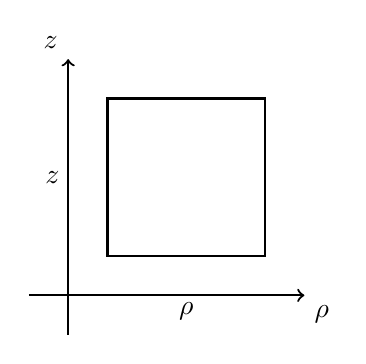
\begin{tikzpicture}
        % Eksenleri çiz
        \draw[thick, ->] (-0.5,0) -- (3,0) node[anchor=north west] {$\rho$};
        \draw[thick, ->] (0,-0.5) -- (0,3) node[anchor=south east] {$z$};

        % Dikdörtgen çiz
        \draw[thick] (0.5,0.5) rectangle (2.5,2.5);
        \node at (1.5, -0.2) {$ \rho $};
        \node at (-0.2, 1.5) {$ z $};
    \end{tikzpicture}
    \caption{$xz$ Düzleminde Dikdörtgen Levha}
    \label{fig:dikdortgen_levha}
\end{figure}

\textbf{2. Döndürme İşlemi:}

Bu levhayı $z$ ekseni etrafında $2\pi$ radyan (360 derece) döndürdüğümüzde, bir silindir elde ederiz. $\phi$ açısı, bu döndürme işlemini temsil eder.

\textbf{3. Silindirin Oluşumu:}

\begin{figure}[htbp]
    \centering
    \begin{tikzpicture}
        % Eksenleri çiz
        \draw[thick, ->] (-3,0) -- (3,0) node[anchor=north west] {x};
        \draw[thick, ->] (0,-3) -- (0,3) node[anchor=south east] {y};
        \draw[thick, ->] (0,0) -- (1.5,1.5) node[anchor=west] {z};

        % Silindir çiz
        \draw[dashed] (1,0) arc (0:360:1);
        \draw[dashed] (1,0) -- (1,2);
        \draw[dashed] (-1,0) -- (-1,2);
        \draw[dashed] (1,2) arc (0:360:1);
    \end{tikzpicture}
    \caption{Silindirik Koordinat Sistemi Oluşumu}
    \label{fig:silindir_olusumu}
\end{figure}

\textbf{4. Sınır Değerleri:}

Silindirik koordinatlarda, her bir değişkenin belirli sınır değerleri vardır:

\begin{itemize}
    \item $\rho$: Yarıçap her zaman pozitif veya sıfır olmalıdır: $\rho \geq 0$.
    \item $\phi$: Azimut açısı genellikle $0$ ile $2\pi$ arasında değişir: $0 \leq \phi < 2\pi$.
    \item $z$: Yükseklik, $-\infty$ ile $+\infty$ arasında herhangi bir değer alabilir: $-\infty < z < +\infty$.
\end{itemize}

\textbf{5. Farklı Döndürme Türleri ve Oluşan Şekiller:}

Eğer levhayı farklı şekillerde döndürürsek, farklı geometrik yapılar elde edebiliriz. Örneğin:

\begin{itemize}
    \item \textbf{Tam Döndürme ($2\pi$)}: $xz$ düzlemindeki dikdörtgenin $z$ ekseni etrafında tam olarak döndürülmesiyle elde edilen silindir.
    \item \textbf{Kısmi Döndürme ($\theta < 2\pi$)}: $xz$ düzlemindeki dikdörtgenin $z$ ekseni etrafında $\theta$ açısı kadar döndürülmesiyle elde edilen silindir parçası.
    \item \textbf{Öteleme}: $xz$ düzlemindeki dikdörtgenin $z$ ekseni boyunca ötelenmesiyle elde edilen prizma.
\end{itemize}

\begin{figure}[htbp]
    \centering
    \begin{tabular}{ccc}
         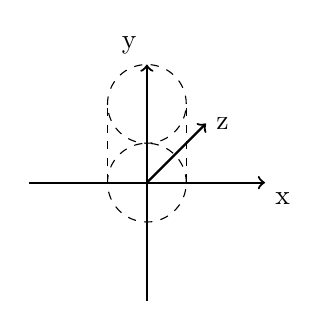
\begin{tikzpicture}[scale=0.5]
        % Eksenleri çiz
        \draw[thick, ->] (-3,0) -- (3,0) node[anchor=north west] {x};
        \draw[thick, ->] (0,-3) -- (0,3) node[anchor=south east] {y};
        \draw[thick, ->] (0,0) -- (1.5,1.5) node[anchor=west] {z};

        % Silindir çiz
        \draw[dashed] (1,0) arc (0:360:1);
        \draw[dashed] (1,0) -- (1,2);
        \draw[dashed] (-1,0) -- (-1,2);
        \draw[dashed] (1,2) arc (0:360:1);
    \end{tikzpicture}
    &
         \begin{tikzpicture}[scale=0.5]
        % Eksenleri çiz
        \draw[thick, ->] (-3,0) -- (3,0) node[anchor=north west] {x};
        \draw[thick, ->] (0,-3) -- (0,3) node[anchor=south east] {y};
        \draw[thick, ->] (0,0) -- (1.5,1.5) node[anchor=west] {z};

        % Silindir çiz
        \draw[dashed] (1,0) arc (0:180:1);
        \draw[dashed] (1,0) -- (1,2);
        \draw[dashed] (-1,0) -- (-1,2);
        \draw[dashed] (1,2) arc (0:180:1);
    \end{tikzpicture}
    &
         \begin{tikzpicture}[scale=0.5]
        % Eksenleri çiz
        \draw[thick, ->] (-3,0) -- (3,0) node[anchor=north west] {x};
        \draw[thick, ->] (0,-3) -- (0,3) node[anchor=south east] {y};
        \draw[thick, ->] (0,0) -- (1.5,1.5) node[anchor=west] {z};

        % Silindir çiz
        \draw[dashed] (1,0) -- (1,2);
        \draw[dashed] (-1,0) -- (-1,2);
        \draw[dashed] (-1,0) -- (1,0);
         \draw[dashed] (-1,2) -- (1,2);
    \end{tikzpicture}
    \\
    Tam Döndürme & Kısmi Döndürme & Öteleme
    \end{tabular}
    \caption{Farklı Döndürme Türleri}
    \label{fig:farkli_dondurme_turleri}
\end{figure}

Bu şemalar, silindirik koordinat sisteminin nasıl oluşturulduğunu ve farklı döndürme türlerinin hangi geometrik yapıları ortaya çıkardığını görsel olarak açıklamaktadır.

\end{document}
\documentclass[11pt,letterpaper,twocolumn]{fenbil}
\usepackage{amsmath}
\usepackage{amssymb}
\usepackage{graphicx}
\usepackage{tikz}
\title{FMM - Fizikte Matematiksel Metotlar - Ders Notları}
\author{Celal Ekrem Torun}
\date{6 Mart 2025}

\begin{document}
\twocolumn[\begin{@twocolumnfalse}

\begin{minipage}{0.15\textwidth}{
    }
\end{minipage}
\hspace{25pt}
\begin{minipage}{0.75\textwidth}
\vspace{5mm}
\Large{\textbf{FMM - Fizikte Matematiksel Metotlar - Ders 1 (6 Mart 2025)}}
    \vspace{3mm}
    
    \large{\textbf{Hazırlayan}; Celal Ekrem Torun}
    \vspace{2mm}
    
    \fontsize{0.35cm}{0.5cm}\selectfont \textit{Fizik Bölümü, İstanbul Üniversitesi\newline 
    Beyazıt, Fatih, İstanbul, Türkiye}
    
\end{minipage}

\small

\end{@twocolumnfalse}]

\section{Matematiksel Metotlar}

\textbf{Not:} 1 Mart'ta gradyen vektörü işlendi, 6 Mart'ta eğrisel koordinatlara başlanacak.

\subsection{Gradyen}

\textbf{Tanım:} Bir $\phi(x, y, z)$ skaler alanının gradyeni, o alanın en hızlı değişim yönünü ve büyüklüğünü gösteren bir vektör alanıdır.

Kartezyen koordinatlarda gradyen şu şekilde tanımlanır:

\[
\nabla \phi = \frac{\partial \phi}{\partial x} \hat{e_x} + \frac{\partial \phi}{\partial y} \hat{e_y} + \frac{\partial \phi}{\partial z} \hat{e_z}
\]

Burada:

\begin{itemize}
    \item $\nabla \phi$: Gradyen vektörü
    \item $\phi(x, y, z)$: Skaler alan
    \item $\hat{e_x}$, $\hat{e_y}$, $\hat{e_z}$: Sırasıyla $x$, $y$ ve $z$ yönlerindeki birim vektörler
\end{itemize}

\textbf{Önemli Not:} $\nabla \phi$, $\hat{e_x}$, $\hat{e_y}$ ve $\hat{e_z}$ ile ayrı ayrı skalar çarpılırsa, $\phi$ fonksiyonunun sınırları ile $x$, $y$ ve $z$ doğrultusundaki değişimi bulunur.

Bir $P(x,y,z)$ noktasındaki $\phi$ fonksiyonunun değişim oranı, $\nabla \phi \cdot d\vec{r}$ ile bulunur. Burada $d\vec{r}$, $P$ noktasından küçük bir yer değiştirmeyi temsil eden vektördür. Eğer $\phi = c_1$ yüzeyinden $\phi = c_2$ yüzeyine gidilirse, değişim $d\phi = c_2 - c_1$ olur ve $d\phi \neq 0$ olur.

Eğer $\nabla \phi \cdot d\vec{r} = d\phi = 0$ ise, $\nabla \phi$, $d\vec{r}$ vektörüne diktir. Bu durumda $\nabla \phi$, $\frac{\nabla \phi}{|\nabla \phi|}$ ile aynı yöndedir.

\subsection{Doğrultu Türevi}

\textbf{Tanım:} Bir $\phi(x,y,z)$ skaler alanının, bir $\vec{u}$ birim vektörü yönündeki doğrultu türevi, $\phi$'nin $\vec{u}$ yönündeki değişim oranını verir.

Doğrultu türevi şu şekilde tanımlanır:

\[
\frac{\partial \phi}{\partial u} = \nabla \phi \cdot \hat{u} = |\nabla \phi| |\hat{u}| \cos \theta
\]

Burada:
\begin{itemize}
    \item $\frac{\partial \phi}{\partial u}$: Doğrultu türevi
    \item $\nabla \phi$: Gradyen vektörü
    \item $\hat{u}$: Birim vektör
    \item $\theta$: $\nabla \phi$ ve $\hat{u}$ arasındaki açı
\end{itemize}

$\frac{\partial \phi}{\partial u}$, $\phi$'nin bir $P(x,y,z)$ noktasındaki $\vec{u}$ birim vektörü ile belirlenen doğrultudaki doğrultu türevidir.

$\frac{\partial \phi}{\partial u} = \nabla \phi \cdot \hat{u} = |\nabla \phi| \cos \theta$

\subsection{Örnek Soru}

$\phi(x, y, z) = x^2yz + 4z^2$ fonksiyonunun $P(1, -2, -1)$ noktasındaki $\vec{dr} = (2\hat{e_x} - \hat{e_y} - 2\hat{e_z})$ doğrultusundaki türevini bulun.

\textbf{Çözüm:}

\textit{Adım 1: Gradyeni hesaplayalım:}

$\nabla \phi = (2xyz) \hat{e_x} + (x^2z) \hat{e_y} + (x^2y + 8z) \hat{e_z}$

\textit{Adım 2: P(1, -2, -1) noktasındaki gradyeni hesaplayalım:}

$\nabla \phi |_P = (2(1)(-2)(-1)) \hat{e_x} + ((1)^2(-1)) \hat{e_y} + ((1)^2(-2) + 8(-1)) \hat{e_z} = 4 \hat{e_x} - \hat{e_y} - 10 \hat{e_z}$

\textit{Adım 3: $\vec{u}$ birim vektörünü bulalım:}

$|\vec{dr}| = \sqrt{2^2 + (-1)^2 + (-2)^2} = \sqrt{9} = 3$

$\hat{u} = \frac{\vec{dr}}{|\vec{dr}|} = \frac{2}{3} \hat{e_x} - \frac{1}{3} \hat{e_y} - \frac{2}{3} \hat{e_z}$

\textit{Adım 4: Doğrultu türevini hesaplayalım:}

$\frac{\partial \phi}{\partial u} = \nabla \phi \cdot \hat{u} = (4 \hat{e_x} - \hat{e_y} - 10 \hat{e_z}) \cdot (\frac{2}{3} \hat{e_x} - \frac{1}{3} \hat{e_y} - \frac{2}{3} \hat{e_z}) = \frac{8}{3} + \frac{1}{3} + \frac{20}{3} = \frac{29}{3} \approx 9.67$

\subsection{Eğrisel Koordinatlar}

Üç boyutlu Öklit uzayında, bir noktanın Kartezyen koordinatları $(x, y, z)$ ile ifade edilir. Şimdi, bu koordinatlara bağlı üç yeni değişken tanımlayalım:

\begin{equation}
u_1 = u_1(x, y, z)
\end{equation}
\begin{equation}
u_2 = u_2(x, y, z)
\end{equation}
\begin{equation}
u_3 = u_3(x, y, z)
\end{equation}

Bu yeni değişkenler, eğrisel koordinatları temsil eder.

\subsubsection{$u_1$, $u_2$, $u_3$'ün Bağımsız Fonksiyonlar Olması}

Lineer homojen bir sistemin sıfırdan farklı çözüme sahip olabilmesi için, katsayılar determinantının sıfıra eşit olması gerekmektedir. Şimdi, $u_1$, $u_2$, $u_3$'ün bağımsız fonksiyonlar olmasının ne anlama geldiğini inceleyelim.

$u_1(x, y, z)$, $u_2(x, y, z)$ ve $u_3(x, y, z)$ fonksiyonları için aşağıdaki ifadeler tanımlanır:

\begin{equation}
u_1 = u_1(x, y, z)
\end{equation}
\begin{equation}
u_2 = u_2(x, y, z)
\end{equation}
\begin{equation}
u_3 = u_3(x, y, z)
\end{equation}

Bu fonksiyonların diferansiyelleri ise şu şekildedir:

\begin{equation}
du_1 = \frac{\partial u_1}{\partial x} dx + \frac{\partial u_1}{\partial y} dy + \frac{\partial u_1}{\partial z} dz
\end{equation}
\begin{equation}
du_2 = \frac{\partial u_2}{\partial x} dx + \frac{\partial u_2}{\partial y} dy + \frac{\partial u_2}{\partial z} dz
\end{equation}
\begin{equation}
du_3 = \frac{\partial u_3}{\partial x} dx + \frac{\partial u_3}{\partial y} dy + \frac{\partial u_3}{\partial z} dz
\end{equation}

Bu denklemleri matris formunda ifade edebiliriz:

\begin{equation}
\begin{bmatrix} du_1 \\ du_2 \\ du_3 \end{bmatrix} = 
\begin{bmatrix}
\frac{\partial u_1}{\partial x} & \frac{\partial u_1}{\partial y} & \frac{\partial u_1}{\partial z} \\
\frac{\partial u_2}{\partial x} & \frac{\partial u_2}{\partial y} & \frac{\partial u_2}{\partial z} \\
\frac{\partial u_3}{\partial x} & \frac{\partial u_3}{\partial y} & \frac{\partial u_3}{\partial z}
\end{bmatrix}
\begin{bmatrix} dx \\ dy \\ dz \end{bmatrix}
\end{equation}

Bu matrisi daha kompakt bir şekilde ifade etmek için, aşağıdaki tanımlamaları yapalım:

\begin{equation}
d\mathbf{u} = \begin{bmatrix} du_1 \\ du_2 \\ du_3 \end{bmatrix}, \quad
A = \begin{bmatrix}
\frac{\partial u_1}{\partial x} & \frac{\partial u_1}{\partial y} & \frac{\partial u_1}{\partial z} \\
\frac{\partial u_2}{\partial x} & \frac{\partial u_2}{\partial y} & \frac{\partial u_2}{\partial z} \\
\frac{\partial u_3}{\partial x} & \frac{\partial u_3}{\partial y} & \frac{\partial u_3}{\partial z}
\end{bmatrix}, \quad
d\mathbf{x} = \begin{bmatrix} dx \\ dy \\ dz \end{bmatrix}
\end{equation}

Bu durumda, yukarıdaki denklem şu şekilde yazılabilir:

\begin{equation}
d\mathbf{u} = A \, d\mathbf{x}
\end{equation}

$dx$, $dy$ ve $dz$'yi $du_1$, $du_2$ ve $du_3$ cinsinden ifade etmek için, $A$ matrisinin tersini almamız gerekir:

\begin{equation}
d\mathbf{x} = A^{-1} \, d\mathbf{u}
\end{equation}

$A^{-1}$ matrisinin var olabilmesi için, $A$ matrisinin determinantı sıfırdan farklı olmalıdır:

\begin{equation}
J = \det(A) \neq 0
\end{equation}

Burada $J$, Jacobian determinantıdır. $A^{-1}$ matrisi, $A$'nın ek matrisinin determinantına bölünmesiyle bulunur:

\begin{equation}
A^{-1} = \frac{\text{adj}(A)}{J}
\end{equation}

Bu durumda, $dx$, $dy$ ve $dz$ aşağıdaki şekilde ifade edilebilir:

\begin{equation}
\begin{bmatrix} dx \\ dy \\ dz \end{bmatrix} = A^{-1} \begin{bmatrix} du_1 \\ du_2 \\ du_3 \end{bmatrix}
\end{equation}

Kartezyen koordinatları eğrisel koordinatlar cinsinden ifade etmek için, aşağıdaki bağıntıları kullanırız:

\begin{equation}
x = x(u_1, u_2, u_3)
\end{equation}
\begin{equation}
y = y(u_1, u_2, u_3)
\end{equation}
\begin{equation}
z = z(u_1, u_2, u_3)
\end{equation}

Bu durumda, konum vektörü $\vec{r}$ aşağıdaki gibi ifade edilir:

\begin{equation}
\vec{r} = x(u_1, u_2, u_3) \, \hat{e_x} + y(u_1, u_2, u_3) \, \hat{e_y} + z(u_1, u_2, u_3) \, \hat{e_z}
\end{equation}

\subsubsection{Eğrisel Koordinatların Geometrik Gösterimi}

Aşağıdaki şemalar, eğrisel koordinatların ve Kartezyen koordinat sisteminin ayrı ayrı gösterimlerini sunmaktadır.

\textbf{Kartezyen Koordinat Sistemi:}

\begin{figure}[htbp]
    \centering
    \begin{tikzpicture}
        \draw[thick, ->] (-3,0) -- (3,0) node[anchor=north west] {x};
        \draw[thick, ->] (0,-3) -- (0,3) node[anchor=south east] {y};
        \draw[thick, ->] (0,0) -- (1.5,1.5) node[anchor=west] {z};
        
        \node[below right] at (2.2, -0.2) {Apsis (x)};
        \node[above] at (-2.2, 0) {Ordinat (y)};
    \end{tikzpicture}
    \caption{Kartezyen Koordinat Sistemi}
    \label{fig:kartezyen_koordinat}
\end{figure}

Bu şemada:

\begin{itemize}
    \item \textit{Apsis (x)}: Yatay ekseni temsil eder.
    \item \textit{Ordinat (y)}: Dikey ekseni temsil eder.
    \item \textit{Kot (z)}: Derinlik eksenini temsil eder.
\end{itemize}

\textbf{Eğrisel Koordinat Sistemi Gösterimi:}

\begin{figure}[htbp]
    \centering
    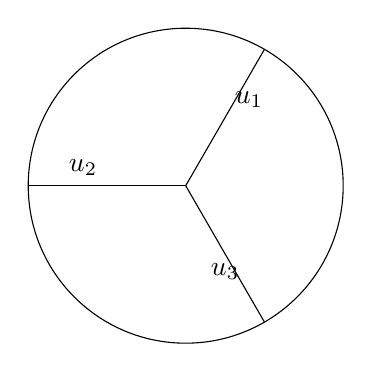
\begin{tikzpicture}
        \draw (0,0) circle (2cm);
        \draw (0,0) -- (60:2cm) node[midway, above right] {$u_1$};
        \draw (0,0) -- (180:2cm) node[midway, above left] {$u_2$};
        \draw (0,0) -- (300:2cm) node[midway, below] {$u_3$};
    \end{tikzpicture}
    \caption{Eğrisel Koordinat Sistemi}
    \label{fig:egrisel_koordinat}
\end{figure}

Bu şema, eğrisel koordinatları $(u_1, u_2, u_3)$ temsil eden bir dairesel gösterim sunar. Bu gösterim, eğrisel koordinatların Kartezyen koordinat sistemi ile ilişkisini anlamak için kullanılabilir.

Eğrisel koordinatlar, belirli bir probleme daha uygun bir koordinat sistemi seçme esnekliği sağlar. Örneğin, silindirik veya küresel koordinatlar, belirli simetrilere sahip problemleri çözmek için daha uygun olabilir.

\subsection{Eğrisel Koordinat Örnekleri}

\subsubsection{Silindirik Koordinatlar $(\rho, \phi, z)$}

Silindirik koordinatlar, üç boyutlu uzayı tanımlamak için kullanılan bir koordinat sistemidir. Bu sistemde, bir noktanın konumu, bir eksene olan uzaklığı $(\rho)$, bu eksen etrafındaki açısı $(\phi)$ ve eksen üzerindeki yüksekliği $(z)$ ile belirlenir.

\textbf{Tanımlar:}

\begin{itemize}
    \item \textit{$\rho$ (rho)}: $xy$ düzlemindeki orijinden olan uzaklık.
    \item \textit{$\phi$ (phi)}: $x$ ekseni ile $\rho$ arasındaki açı (azimut açısı).
    \item \textit{$z$}: $z$ ekseni üzerindeki yükseklik.
\end{itemize}

\textbf{Kartezyen ve Silindirik Koordinatlar Arasındaki İlişki:}

Kartezyen koordinatlardaki $(x, y, z)$ noktası ile silindirik koordinatlardaki $(\rho, \phi, z)$ noktası arasındaki dönüşüm aşağıdaki gibidir:

\begin{itemize}
    \item $x = \rho \cos \phi$
    \item $y = \rho \sin \phi$
    \item $z = z$
\end{itemize}

\textbf{Dönüşümün Tersi:}

\begin{itemize}
    \item $\rho = \sqrt{x^2 + y^2}$
    \item $\phi = \arctan \left( \frac{y}{x} \right)$
    \item $z = z$
\end{itemize}

\textbf{Geometrik Gösterim:}

\begin{figure}[htbp]
    \centering
    \begin{tikzpicture}
        % Eksenleri çiz
        \draw[thick, ->] (-3,0) -- (3,0) node[anchor=north west] {x};
        \draw[thick, ->] (0,-3) -- (0,3) node[anchor=south east] {y};
        \draw[thick, ->] (0,0) -- (1.5,1.5) node[anchor=west] {z};

        % Silindir çiz
        \draw[dashed] (1,0) arc (0:360:1);
        \draw[dashed] (1,0) -- (1,2);
        \draw[dashed] (-1,0) -- (-1,2);
        \draw[dashed] (1,2) arc (0:360:1);

        % P noktası
        \node[circle, fill, inner sep=1.5pt, label=above right:$P$] (P) at (0.7, 1, 1) {};

        % P' noktası
        \node[circle, fill, inner sep=1.5pt, label=below:$P'$] (Pp) at (0.7,0,0) {};

        % rho
        \draw[dashed] (0,0) -- (Pp) node[midway, below] {$\rho$};

        % z
        \draw[dashed] (Pp) -- (P) node[midway, right] {$z$};

        % Açı phi
        \draw (0.4,0) arc (0:45:0.4);
        \node at (0.7,0.3) {$\phi$};

    \end{tikzpicture}
    \caption{Silindirik Koordinat Sistemi}
    \label{fig:silindirik_koordinat}
\end{figure}

Bu şemada:

\begin{itemize}
    \item $P$: Uzaydaki bir noktayı temsil eder.
    \item $P'$: $P$ noktasının $xy$ düzlemindeki izdüşümüdür.
    \item $\rho$: $P'$ noktasının orijine olan uzaklığıdır.
    \item $\phi$: $x$ ekseni ile $OP'$ arasındaki açıdır (azimut açısı).
    \item $z$: $P$ noktasının $z$ ekseni üzerindeki yüksekliğidir.
\end{itemize}

\textbf{Jacobian Dönüşümü:}

Silindirik koordinatlardaki $(\rho, \phi, z)$ ile Kartezyen koordinatlardaki $(x, y, z)$ arasındaki ilişki aşağıdaki gibidir:

\begin{itemize}
    \item $x = \rho \cos \phi$
    \item $y = \rho \sin \phi$
    \item $z = z$
\end{itemize}

Burada $\phi$, azimut açısını temsil etmektedir.

Bu dönüşümü ifade etmek için Jacobian matrisini kullanabiliriz. Jacobian matrisi, koordinat dönüşümünün kısmi türevlerini içerir:

\begin{equation}
J = \begin{bmatrix}
\frac{\partial x}{\partial \rho} & \frac{\partial x}{\partial \phi} & \frac{\partial x}{\partial z} \\
\frac{\partial y}{\partial \rho} & \frac{\partial y}{\partial \phi} & \frac{\partial y}{\partial z} \\
\frac{\partial z}{\partial \rho} & \frac{\partial z}{\partial \phi} & \frac{\partial z}{\partial z}
\end{bmatrix}
\end{equation}

Bu matrisin elemanlarını hesaplarsak:

\begin{itemize}
    \item $\frac{\partial x}{\partial \rho} = \cos \phi$
    \item $\frac{\partial x}{\partial \phi} = -\rho \sin \phi$
    \item $\frac{\partial x}{\partial z} = 0$
    \item $\frac{\partial y}{\partial \rho} = \sin \phi$
    \item $\frac{\partial y}{\partial \phi} = \rho \cos \phi$
    \item $\frac{\partial y}{\partial z} = 0$
    \item $\frac{\partial z}{\partial \rho} = 0$
    \item $\frac{\partial z}{\partial \phi} = 0$
    \item $\frac{\partial z}{\partial z} = 1$
\end{itemize}

Bu değerleri Jacobian matrisine yerleştirdiğimizde:

\begin{equation}
J = \begin{bmatrix}
\cos \phi & -\rho \sin \phi & 0 \\
\sin \phi & \rho \cos \phi & 0 \\
0 & 0 & 1
\end{bmatrix}
\end{equation}

Jacobian determinantı ise şu şekilde hesaplanır:

\begin{equation}
\det(J) = \rho \cos^2 \phi + \rho \sin^2 \phi = \rho (\cos^2 \phi + \sin^2 \phi) = \rho
\end{equation}

Burada $\rho = \sqrt{x^2 + y^2}$ ve $\rho \neq 0$ olmalıdır.

Ayrıca, $\phi = \arctan \left( \frac{y}{x} \right)$ ifadesi kullanılır.

$z = z$ olduğundan, $z$ için türev dönüşümleri basittir.

Bu Jacobian determinantı, hacim elemanının dönüşümünde kullanılır:

\begin{equation}
dV = dx \, dy \, dz = |J| \, d\rho \, d\phi \, dz = \rho \, d\rho \, d\phi \, dz
\end{equation}

Bu dönüşümler, koordinatları bir sistemden diğerine dönüştürmek için kullanılır. Jacobian determinantı, dönüşümün hacim elemanını nasıl etkilediğini gösterir.

\textbf{Silindirik Koordinatların Oluşumu ve Sınır Değerleri}

Silindirik koordinat sistemi, bir levhanın (dikdörtgenin) bir eksen etrafında döndürülmesiyle görselleştirilebilir. Bu bölümde, bu dönüşümün nasıl gerçekleştiğini ve silindirik koordinatların sınır değerlerini inceleyeceğiz.

\textbf{1. Levhanın (Dikdörtgenin) Çizimi:}

İlk olarak, $xz$ düzleminde bir levha (dikdörtgen) çizelim. Bu levha, silindirin yüksekliğini $(z)$ ve yarıçapını $(\rho)$ temsil edecektir.

\begin{figure}[htbp]
    \centering
    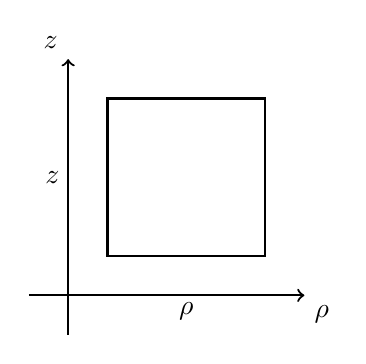
\begin{tikzpicture}
        % Eksenleri çiz
        \draw[thick, ->] (-0.5,0) -- (3,0) node[anchor=north west] {$\rho$};
        \draw[thick, ->] (0,-0.5) -- (0,3) node[anchor=south east] {$z$};

        % Dikdörtgen çiz
        \draw[thick] (0.5,0.5) rectangle (2.5,2.5);
        \node at (1.5, -0.2) {$ \rho $};
        \node at (-0.2, 1.5) {$ z $};
    \end{tikzpicture}
    \caption{$xz$ Düzleminde Dikdörtgen Levha}
    \label{fig:dikdortgen_levha}
\end{figure}

\textbf{2. Döndürme İşlemi:}

Bu levhayı $z$ ekseni etrafında $2\pi$ radyan (360 derece) döndürdüğümüzde, bir silindir elde ederiz. $\phi$ açısı, bu döndürme işlemini temsil eder.

\textbf{3. Silindirin Oluşumu:}

\begin{figure}[htbp]
    \centering
    \begin{tikzpicture}
        % Eksenleri çiz
        \draw[thick, ->] (-3,0) -- (3,0) node[anchor=north west] {x};
        \draw[thick, ->] (0,-3) -- (0,3) node[anchor=south east] {y};
        \draw[thick, ->] (0,0) -- (1.5,1.5) node[anchor=west] {z};

        % Silindir çiz
        \draw[dashed] (1,0) arc (0:360:1);
        \draw[dashed] (1,0) -- (1,2);
        \draw[dashed] (-1,0) -- (-1,2);
        \draw[dashed] (1,2) arc (0:360:1);
    \end{tikzpicture}
    \caption{Silindirik Koordinat Sistemi Oluşumu}
    \label{fig:silindir_olusumu}
\end{figure}

\textbf{4. Sınır Değerleri:}

Silindirik koordinatlarda, her bir değişkenin belirli sınır değerleri vardır:

\begin{itemize}
    \item $\rho$: Yarıçap her zaman pozitif veya sıfır olmalıdır: $\rho \geq 0$.
    \item $\phi$: Azimut açısı genellikle $0$ ile $2\pi$ arasında değişir: $0 \leq \phi < 2\pi$.
    \item $z$: Yükseklik, $-\infty$ ile $+\infty$ arasında herhangi bir değer alabilir: $-\infty < z < +\infty$.
\end{itemize}

\textbf{5. Farklı Döndürme Türleri ve Oluşan Şekiller:}

Eğer levhayı farklı şekillerde döndürürsek, farklı geometrik yapılar elde edebiliriz. Örneğin:

\begin{itemize}
    \item \textbf{Tam Döndürme ($2\pi$)}: $xz$ düzlemindeki dikdörtgenin $z$ ekseni etrafında tam olarak döndürülmesiyle elde edilen silindir.
    \item \textbf{Kısmi Döndürme ($\theta < 2\pi$)}: $xz$ düzlemindeki dikdörtgenin $z$ ekseni etrafında $\theta$ açısı kadar döndürülmesiyle elde edilen silindir parçası.
    \item \textbf{Öteleme}: $xz$ düzlemindeki dikdörtgenin $z$ ekseni boyunca ötelenmesiyle elde edilen prizma.
\end{itemize}

\begin{figure}[htbp]
    \centering
    \begin{tabular}{ccc}
         \begin{tikzpicture}[scale=0.5]
        % Eksenleri çiz
        \draw[thick, ->] (-3,0) -- (3,0) node[anchor=north west] {x};
        \draw[thick, ->] (0,-3) -- (0,3) node[anchor=south east] {y};
        \draw[thick, ->] (0,0) -- (1.5,1.5) node[anchor=west] {z};

        % Silindir çiz
        \draw[dashed] (1,0) arc (0:360:1);
        \draw[dashed] (1,0) -- (1,2);
        \draw[dashed] (-1,0) -- (-1,2);
